% Format teze zasnovan je na paketu memoir
% http://tug.ctan.org/macros/latex/contrib/memoir/memman.pdf ili
% http://texdoc.net/texmf-dist/doc/latex/memoir/memman.pdf
% 
% Prilikom zadavanja klase memoir, navedenim opcijama se podešava 
% veličina slova (12pt) i jednostrano štampanje (oneside).
% Ove parametre možete menjati samo ako pravite nezvanične verzije
% mastera za privatnu upotrebu (na primer, u b5 varijanti ima smisla 
% smanjiti 
\documentclass[12pt,oneside]{memoir} 

% Paket koji definiše sve specifičnosti master rada Matematičkog fakulteta
\usepackage[latinica]{matfmaster} 
%
% Podrazumevano pismo je ćirilica.
%   Ako koristite pdflatex, a ne xetex, sav latinički tekst na srpskom jeziku
%   treba biti okružen sa \lat{...} ili \begin{latinica}...\end{latinica}.
%
% Opicija [latinica]:
%   ako želite da pišete latiniciom, dodajte opciju "latinica" tj.
%   prethodni paket uključite pomoću: \usepackage[latinica]{matfmaster}.
%   Ako koristite pdflatex, a ne xetex, sav ćirilički tekst treba biti
%   okružen sa \cir{...} ili \begin{cirilica}...\end{cirilica}.
%
% Opcija [biblatex]:
%   ako želite da koristite reference na više jezika i umesto paketa
%   bibtex da koristite BibLaTeX/Biber, dodajte opciju "biblatex" tj.
%   prethodni paket uključite pomoću: \usepackage[biblatex]{matfmaster}
%
% Opcija [b5paper]:
%   ako želite da napravite verziju teze u manjem (b5) formatu, navedite
%   opciju "b5paper", tj. prethodni paket uključite pomoću: 
%   \usepackage[b5paper]{matfmaster}. Tada ima smisla razmisliti o promeni
%   veličine slova (izmenom opcije 12pt na 11pt u \documentclass{memoir}).
%
% Naravno, opcije je moguće kombinovati.
% Npr. \usepackage[b5paper,biblatex]{matfmaster}

% Pomoćni paket koji generiše nasumičan tekst u kojem se javljaju sva slova
% azbuke (nema potrebe koristiti ovo u pravim disertacijama)
\usepackage[latinica]{pangrami}
\usepackage{subfig}
\usepackage{float}
% Datoteka sa literaturom u BibTex tj. BibLaTeX/Biber formatu
\bib{matfmaster-primer}

% Ime kandidata na srpskom jeziku (u odabranom pismu)
\autor{Lazar Čeliković}
% Naslov teze na srpskom jeziku (u odabranom pismu)
\naslov{Upravljanje razvojem mobilnih aplikacija sa fokusom na performanse i kvalitet}
% Godina u kojoj je teza predana komisiji
\godina{2024}
% Ime i afilijacija mentora (u odabranom pismu)
\mentor{dr Vladimir \textsc{Filipović}, redovan profesor\\ Univerzitet u Beogradu, Matematički fakultet}
% Ime i afilijacija prvog člana komisije (u odabranom pismu)
\komisijaA{dr Aleksandar \textsc{Kartelj}, vanredni profesor\\ Univerzitet u Beogradu, Matematički fakultet}
% Ime i afilijacija drugog člana komisije (u odabranom pismu)
\komisijaB{dr Staša \textsc{Vujučić Stanković}, docent\\ Univerzitet u Beogradu, Matematički fakultet}
% Ime i afilijacija trećeg člana komisije (opciono)
% \komisijaC{}
% Ime i afilijacija četvrtog člana komisije (opciono)
% \komisijaD{}
% Datum odbrane (odkomentarisati narednu liniju i upisati datum odbrane ako je poznat)
% \datumodbrane{}

% Apstrakt na srpskom jeziku (u odabranom pismu)
\apstr{%
Mobilne aplikacije i aplikacije generalno često se razvijaju sa primarnim ciljem da se pokrije što je moguće više funkcionalnosti, dok se koncepti kao što su performanse zanemaruju dok problem ne postane evidentan. U ovom radu se razmatra pristup koji ove koncepte stavlja u središte i implementira ih na samom početku razvojnog ciklusa. Rad prikazuje kako postavljanje sistema za merenje performansi, poslovnih metrika i analizu grešaka olakšava dalji razvoj u kasnijim stadijumima projekta. Rešenje koje ćemo analizirati razvijeno je uz pomoć razvojnog okruženja ReactNative uz podršku RTKQ biblioteke sa menadžovanje stanja podataka. Rad prikazuje detalje implementacije ovih sistema kao i benefite koje dobijamo korišćenjem istih. Pomenuti koncepti biće prikazani i analizirani na primeru mobilne aplikacije za vremensku prognozu.
}

% Ključne reči na srpskom jeziku (u odabranom pismu)
\kljucnereci{mobilna aplikacija, performanse, dogadjaji, računarstvo, programiranje}

\begin{document}
% ==============================================================================
% Uvodni deo teze
\frontmatter
% ==============================================================================
% Naslovna strana
\naslovna
% Strana sa podacima o mentoru i članovima komisije
\komisija
% Strana sa posvetom (u odabranom pismu)
% Strana sa podacima o disertaciji na srpskom jeziku
\apstrakt
% Sadržaj teze
\tableofcontents*

% ==============================================================================
% Glavni deo teze
\mainmatter
% ==============================================================================

% ------------------------------------------------------------------------------
\chapter{Uvod}
% ------------------------------------------------------------------------------

% ------------------------------------------------------------------------------
\chapter{Pregled tehnologija za razvoj mobilnih aplikacija}
\label{chp:pregledTehnologijaZaRazvojMobilnihAplikacija}

% ------------------------------------------------------------------------------
Mobilne aplikacije su doživele neverovatnu evoluciju od svog početka. Svedoci smo kako su one iz jednostavnih alata za komunikaciju ili zabavu prerastle u složene sisteme koji nam pomažu u svakodnevnom životu. Danas, aplikacije nisu samo način da ostanemo povezani s drugima, već i sredstvo za upravljanje finansijama, učenje novih veština, pa čak i za praćenje zdravlja i fitnessa. Razvoj tehnologija poput veštačke inteligencije i mašinskog učenja dodatno je unapredio funkcionalnost i intuitivnost aplikacija, pružajući korisnicima personalizovano iskustvo koje je prethodnih godina bilo nezamislivo. Ovaj napredak ne samo da je promenio način na koji interagujemo sa našim uređajima, već je i potpuno preoblikovao digitalni pejzaž, otvarajući nove mogućnosti za razvoj i inovacije u budućnosti. Ovaj napredak mobilnih aplikacija pratio je i razvoj tehnologija koje se koriste u izradi istih. Kroz vreme, došli smo do većeg broja tipova mobilnih aplikacija kao i do velikog broja radnih okvira koji nam omogućavaju lakši razvoj i održavanje aplikacija na kojima radimo.

\section{Tipovi mobilnih aplikacija}

Mobilne aplikacije mogu se kategorisati u nekoliko osnovnih tipova, svaki sa svojim specifičnim funkcijama i ciljevima. Delimo ih na nativne aplikacije(eng. native mobile applications), veb aplikacije (eng. web mobile applications), hibridne mobilne aplikacije i progrsivne veb alikacije (eng. progressive web applications - (PWA)). Svaki od ovih tipova ima svoje prednosti i mane, te izbor tipa aplikacije zavisi od specifičnih potreba i ciljeva projekta. U nastavku rada ćemo analizirati svaku od pomenutih kategorija.

\subsection{Nativne mobilne aplikacije}

Nativne mobilne aplikacije (eng. native mobile applications) su programi razvijeni za specifičan operativni sistem, kao što je iOS ili Android, koristeći programerske jezike koji su specifični za svaku od platformi. Tako imamo Swift i Objective C za iOS ili Kotlin i Javu za Android. Ove aplikacije se instaliraju direktno na mobilni uređaj preko prodavnice aplikacija na uređaju i optimizovane su da pružaju maksimalnu efikasnost i iskoristivost hardverskih karakteristika uređaja. Prednsoti ovog tipa mobilnih aplikacija su:

\begin{itemize}
    \item Budući da je ovaj tip aplikacija optimizovan za specifičnu platformu, po pravilu se mogu izvući neuporedivo više performanse u poređenju sa ostalim tipovima.
    \item Fluidne animacije i intuitivan interfejs koji potiče od samog operativnog sistema rezultuju poboljšanim korisničkim iskustvom.
    \item Mogućnost pristupa punom setu hardverskih i softverskih funkcija samog uređaja kao što su kamera, GPS, senzori
    \item Nativne mobilne aplikacije se objavljuju na prodavnicama aplikacija kao sto su Play prodavnica (eng. Play Store) i App prodavnica (eng. App store). Tokom ovog procesa se vrši detaljno ispitivanje aplikacija i na ovaj način se povećava sigurnost.
\end{itemize}
Mane ovog tipa mobilnih aplikacija su:
\begin{itemize}
    \item Razvijanje posebne aplikacija za svaki operativni sistem povećava troškove kao i vreme koje je potrebno da se aplikacija pusti u korišćenje
    \item Različiti operativni sistemi često iziskuju različite programske jezike za razvoj, što može otežati pronalaženje razvojnih timova.
    \item Svaka promena ili ažuriranje aplikacija zahteva odvojeno slanje na odobrenje prodavnicu aplikacija za svaki operativni sistem. Ovaj proces je često vremenski zahtevan.
\end{itemize}

\begin{figure}[h]
    \centering
    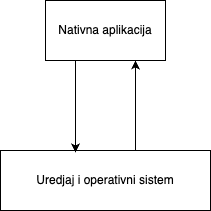
\includegraphics[scale=0.5]{docs/images/chapterTwo/nativnaAplikacija.png}
    \caption{Komunikacija nativne aplikacije i operativnog sistema}
    \label{fig:nativnaAplikacija}
\end{figure}

\subsection{Veb aplikacije}

Veb aplikacije (eng. web applications) su pristupačne preko internet pretraživača i ne zahtevaju preuzimanje i instalaciju na uređaj kao tradicionalne aplikacije. One su dizajnirane da budu kompatibilne sa različitim platformama i pružaju jedinstveno iskustvo korisnicima na različitim uređajima. One predstavljaju korisnu opciju za aplikacije koje zahtevaju brzu dostupnost i lako održavanje, ali kada je u pitanju duboka integracija sa uređajem i složene interakcije, ovaj tip aplikacije često zaostaje za mogućnostima koje pružaju nativne aplikacije. Prednosti veb mobilnih aplikacija:

\begin{itemize}
    \item Ovaj tip mobilnih aplikacija će raditi na bilo kom uređaju koji ima veb pretraživač. Ova osobina uklanja potrebu za posebnim verzijama za različite operativne sisteme.
    \item Ovaj tip mobilnih aplikacija razvija se samo jednom za sve platforme, čime se troškovi razvoja i ažuriranja značajno smanjuju u odnosu na nativne aplikacije.
    \item Korisnici veb aplikacija imaće pristup najnovijim izmenama onog momenta kada te izmene budu puštene na produkciju. Ovo znači da se uklanja potreba za preuzimanjem ažururanja, što znatno olakšava distribuciju i održavanje.
\end{itemize}
Mane ovog tipa mobilnih aplikacija su:
\begin{itemize}
    \item Veb mobilne aplikacije zavise od brzine i kvaliteta internet konekcije, a takođe ne mogu u potpunosti iskoristiti sve hardverske mogućnosti uređaja kao što to mogu nativne mobilne aplikacije.
    \item Korisnički interfejsi ovog tipa mobilnih aplikacija često su manje fluidni i intuitivni u odnosu na nativne mobilne aplikacije, što može uticati na ukupno korisničko iskustvo.
    \item Funkcionalnosti i performanse mogu varirati u zavisnosti od pretraživača koji korisnik upotrebljava, što može rezultovati u nekonzistentnosti u korisničkom iskustvu.
\end{itemize}

\begin{figure}[h]
    \centering
    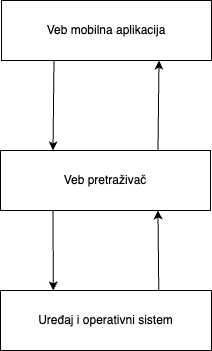
\includegraphics[scale=0.5]{docs/images/chapterTwo/vebMobilnaAplikacija.png}
    \caption{Komunikacija veb aplikacije i operativnog sistema}
    \label{fig:vebMobilnaAplikacija}
\end{figure}

\subsection{Progresivne veb mobilne aplikacije}

Progresivne veb aplikacije (eng. Progressive Web Applications (PWA)) su vrsta aplikacija koje kombinuju najbolje osobine tradicionalnih veb aplikacija i native mobilnih aplikacija. One se izvršavaju u veb pretraživaču, ali pružaju korisničko iskustvo koje je blisko iskustvu koje pružaju nativne mobilne aplikacije. PWA su dizajnirane da budu brze, pouzdane, čak i u uslovima loše internet konekcije. Osnovne prednosti ovog tipa aplikacija su:

\begin{itemize}
    \item Zahvaljujući servisnim radnicima (eng. service workers), progresivne veb aplikacije mogu raditi offline ili na slabim mrežnim konekcijama, pružajući osnovnu funkcionalnost kada nema internet konekcije.
    \item Korisnici mogu "instalirati" progresivne veb aplikacije na svoje uređaje, omogućavajući im da pristupe aplikaciji sa početnog ekrana, slično kao kod nativnih aplikacija.
    \item Progresivne veb aplikacije imaju podršku za notifikacija (eng. push notification), što omogućava bolje zadržavanje korisnika (eng. retention).
    \item Progresivne veb aplikacije zahtevaju HTTPS\footnote{eng. Hypertext transfer protocol secure} za pokretanje, što omogućava sigurniju razmenu podataka između korisnika i aplikacije.
\end{itemize}
Mane ovog tipa mobilnih aplikacija su:
\begin{itemize}
    \item Iako progresivne veb aplikacije imaju pristup nekim hardverskim funkcijama, one ne mogu potpuno iskoristiti sve kapacitete uređaja kao što to mogu nativne aplikacije.
    \item Ovaj tip aplikacija nije jednako podržan na svim platformama, s iOS uređajima koji imaju određena ograničenja u pogledu funkcionalnosti u odnosu na Android uređaje.
    \item Razvoj ovog tipa mobilnih aplikacija može biti složeniji od tradicionalnih veb aplikacija zbog potrebe za implementacijom servisnih radnika i upravljanjem keširanim podacima za offline rad.
\end{itemize}

U poređenju sa tradicionalnim web aplikacijama, PWA pružaju bolje korisničko iskustvo, veću pouzdanost i više funkcionalnosti koje su bliske native iskustvu, čineći ih izuzetno privlačnim izborom za razvoj aplikacija koje treba da budu efikasne i dostupne širom različitih platformi i uslova povezivanja.

\subsection{Hibridne mobilne aplikacije}

Hibridne mobilne aplikacije (eng. crossplatform mobile application) predstavljaju spoj nativnih i veb tehnologija, omogućavajući razvoj aplikacija koje se mogu instalirati na uređaj, ali se izvršavaju u veb kontejneru. Ove aplikacije koriste kombinaciju HTML, CSS, i JavaScript za izradu korisničkog interfejsa, dok istovremeno koriste mostove (eng. bridge) poput Cordova ili Ionic za pristup native funkcijama uređaja. Ovaj tip aplikacije biće implementiran u okviru ovog rada pa ćemo imati prilike detaljnije da se upoznamo sa karaktiristikama istih. Osnovne prednosti ovog tipa mobilnih aplikacija su:

\begin{itemize}
    \item Razvoj se vrši koristeći veb tehnologije koje su mnogim programerima već poznate, što smanjuje vreme i troškove razvoja.
    \item Jedan kod može se koristiti za više platformi (iOS, Android, Windows Phone), što dodatno smanjuje troškove i olakšava održavanje.
    \item Kroz različite biblioteke, hibridne mobilne aplikacije mogu koristiti hardver uređaja (kamere, GPS, senzore i druge funkcije).
\end{itemize}
Mane ovog tipa mobilnih aplikacija su:
\begin{itemize}
    \item Zbog dodatnog sloja apstrakcije i oslanjanja na veb tehnologije, performanse hibridnih aplikacija mogu biti lošije u odnosu na nativne aplikacije, posebno za zahtevne zadatke. Ovo je idealan razlog zbog koga bi trebalo razmotriti implementiranje sistema za praćenje performansi na početku razvoja aplikacije.
    \item Iako se ne trude da imitiraju izgled i osećaj nativnih aplikacija, hibridne mobilne aplikacije često ne mogu potpuno replicirati fludinost i odziv nativnog korisničkog interfejsa.
    \item Ovaj tip mobilnij aplikacija zavisi od platformi kao što su Cordova ili Ionic, što može dovesti do problema ako se ti alati ne ažuriraju redovno ili ne podržavaju najnovije verzije operativnih sistema.
\end{itemize}

\begin{figure}[h]
    \centering
    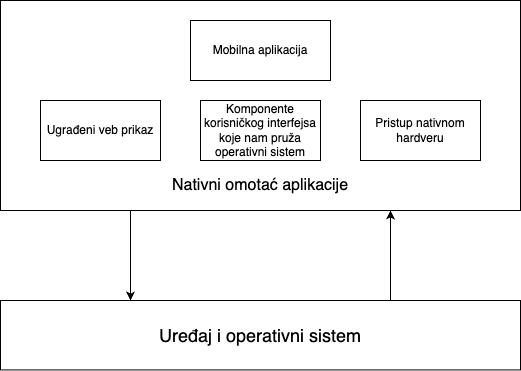
\includegraphics[scale=0.5]{docs/images/chapterTwo/hibridnaMobilnaAplikacija.png}
    \caption{Komunikacija hibridne mobilne aplikacije i operativnog sistema}
    \label{fig:hibridnaMobilnaAplikacija}
\end{figure}

\chapter{Osnove radnog okvira React Native}

React Native (eng. React Native) predstavlja JavaScript radni okvir (eng. framework) za kreiranje mobilnih aplikacija za iOS i Android operativne sisteme. Zasnovan je na React radnom okviru, sa izmenom da targetuje mobilne uređaje. Dakle, ovaj radni okvir omogućava nam da kreiramo mobilne aplikacije koje imaju nativni izgled kao i korisničko iskustvo, a sve to korišćenjem dobro poznatih veb tehnologija. React Native razvijen je 2015. godine od strane kompanije Meta Inc., ranije poznata kao Facebook Inc. Od tada, sam radni okvir se dosta izmenio i postao je jedan od najpopularnijih alata za ravoj mobilnih aplikacija.

\section{Kako React Native zapravo radi}

Osnovna ideja iza ovog radnog okvira jeste da kombinuje dve zasebne celine - JavaScript kod sa jedne i nativni kod sa druge strane (Java/Kotlin za Android i Ojective-C/Swift za iOS) i učini da njih dve međusobno sarađuju. Nativni kod će se izvršavati na samom uređaju, dok će za JavaScript kod biti neophodna virtuelna mašina. Ovo nam nije problematično na iOS uređajima iz razloga što oni poseduju ugrađeni JavaScript pokretač nazvan JavaScriptCore. Android uređaji nemaju ugrađen ovaj pokretač, međutim React Native se brine za to i on donosi isto za Android uređaje. Napomenućemo ovde da ovo rezultuje time da se veličina same aplikacije povećava za Android.

\subsection{Komunikacija između uređaja i JavaScript-a}

Kako se programski jezici koji se koriste na samim uređajima razlikuju od JavaScript programskog jezika neophodno je da se kreira neki protokol kako bi oni mogli međusobno da komuniciraju. Ovo se postiže preko formata koji obe strane razumeju, a to je JSON. Sva komunikacija između ovih delova sistema obavlja se preko mosta (eng. Bridge).

\subsection{Niti korišćene u React Native radnom okviru}

Kada korisnik pokrene React Native aplikaciju, sam uređaj će kreirati tri glavne niti i ostale ukoliko za istim postoji potreba. Niti koje će biti kreirane su Glavna nit (eng. Main Thread), JavaScript nit (eng. JavaScript thread) i nit u senci (eng. Shadow Thread).

\begin{itemize}
    \item Glavna nit (eng. Main Thread) - ova nit poznata je i kao nit korisničkog interfejsa. To je osnovna nit svaki iOS ili Android aplikacije i predstavlja glavnu nativnu nit na kojoj će se naša aplikacije izvršavati. Njena odgovornost jeste da obrađuje korisničke interakcije sa uređajem kao i da ažurira sam korisnički interfejs na ekranu uređaja. U React Native radnom okviru sve nativne komponente se renderuju na ovoj niti i iz ovog razloga je veoma bitno da se izbegavaju složene operacije na ovoj niti kako ne bi došlo do blokiranja korisničkog interfejsa i smanjenja performansi.
    \item JavaScript nit (eng. JavaScript Thread) - na ovoj niti će se izvršavati sav JavaScript i React kod naše aplikacije. Ona obrađuje logiku aplikacije, API pozive, vrši proračune i upravlja stanjem aplikacije. Ova nit je ključna za sve što nije povezano sa korisničkim interfejsom. Ova nit radi zasebno od glavne niti što nam omogućava da radimo kompleksna izračunavanja bez da blokiramo glavnu nit. 
    \item Nit u senci (eng. Shadow Thread) - ova nit poznata je jos i kao nit rasoreda (eng. Layout Thread) . Odgovornost ove niti jeste da preračunava pozicije elemenata i da generiše stablo za prikazivanje koje je kodirano u JavaScript niti. Kada se ovo izračunavanje završi ti podaci se šalju glavnoj niti koja vrši prikazivanje. Njena uloga jeste da oslobodi glavnu nit ovog posla, koji može biti veoma zahtevan. Ovaj pristup nam omogućava da imamo fluidno korisničko iskustvo.
\end{itemize}

\begin{figure}[h]
    \centering
    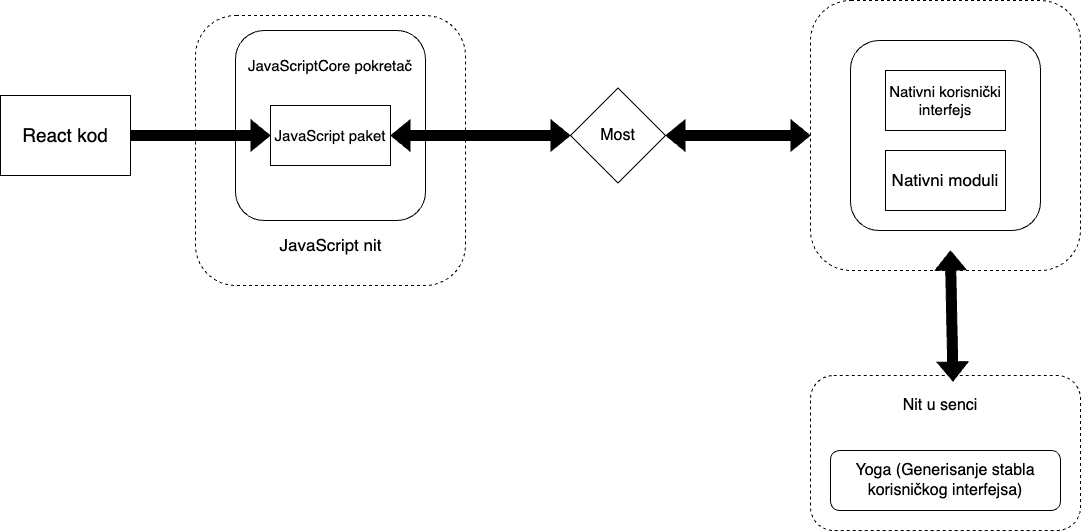
\includegraphics[scale=0.4]{docs/images/chapterThree/reactNativeArchitecture.png}
    \caption{Arhitektura React Native radnog okvira}
    \label{fig:reactNativeArchitecture}
\end{figure}

\section{Most u React Native radnom okviru}

U arhitekturi radnog okvira React Native, most (eng. bridge) igra ključnu ulogu u omogućavanju komunikacije između JavaScript niti i nativnih delova aplikacije koji se izvršavaju na glavnoj niti. Ovaj most funkcioniše kao posrednik koji prenosi informacije između dve sredine koje inače ne bi mogle direktno da komuniciraju zbog različitih programskih jezika (JavaScript sa jedne i Objective-C i Java sa druge strane). Komunikacija se obalja asinhronom razmenom JSON poruka izmedju ova dva okruženja. JavaScript kod se izvršava u svom okruženju, dok se nativne komponente upravljaju kroz specifične platforme kao što su iOS ili Android. Most omogućava asinhronu komunikaciju između ova dva okruženja prenošenjem poruka, što znači da informacije mogu preći iz jednog okruženja u drugo bez blokiranja glavne niti ili usporavanja aplikacije. Kada JavaScript kod zahteva pristup nativnim funkcionalnostima (kao što su pristup kameri ili GPS-u) ili kada treba da se ažurira korisnički interfejs, most prenosi ove zahteve iz JavaScript-a u nativni sistem, i obratno, prenosi odgovore nazad. Ovaj mehanizam omogućava React Native aplikacijama da koriste prednosti kako veb tehnologija, tako i nativnih performansi, iako ponekad može predstavljati usko grlo u performansama ako se prevelik broj zahteva mora preneti preko mosta.

\begin{figure}[h]
    \centering
    
\includegraphics[scale=0.5]{docs/images/chapterThree/reactNativeBridge.png}
    \caption{Funkcionisanje mosta}
    \label{fig:reactNativeBridge}
\end{figure}

\subsection{Primer rada mosta}

Sada ćemo proći kroz primer kako most izvodi komunikaciju između nativnog dela i JavaScript dela mobilne aplikacije.

\begin{enumerate}
    \item Okida se nativni događaj. Recimo da je u pitanju klik na dugme.
    \item Serijalizovana poruka šalje se sa nativne strane kroz most sa svim neophodnim podacima
    \item JavaScript prima poruku, deserijalizuje je i odlučuje šta je sledeći korak koji je potrebno preduzeti. U ovom slučaju to je akcija koja je pridružena dugmetu.
    \item Šalje se poruka sa JavaScript strane kroz most sa svim potrebnim informacijama vezanima za traženu akciju.
    \item Nativna strana prima poruku, deserijalizuje je i vrši ponovno renderovanje korisničkog interfejsa.
\end{enumerate}

\subsection{Nedostaci mosta}

Asinhrona priroda prenosa poruka između nativnog i JavaScript dela mobilne aplikacija dovodi do problema koji se manifestuju u ivičnim slučajevima. Na primer, pretpostavimo da imamo polje za unos teksta gde korisnik unosi broj kartice. Želimo da formatiramo taj unos tako što ćemo ubaciti prazan karakter posle svakog četvrtog karaktera u kartici. Ova logika biće implementirana na JavaScript strani. Problem koji se ovde uočava jeste taj da kada korisnik pritisne peti broj po redu nativna strana aplikacije to javlja JS strani. Broj se nadovezuje na prethodni broj kartice i to se javlja nativnoj strani koja će ovo prikazati. Ovo dovodi do toga da će prvo biti renderovan broj bez razmaka, a tek kasnije će se izvršiti formatiranje i preko mosta će biti poslata sledeća poruka koja će nativnoj strani reći da treba da renderuje i razmak. Naravno, ukoliko most nije previše opterećen u tom momentu korisnik ne bi mogao da primeti ovo. Međutim, u situaciji kada se ogroman broj operacija izvršava paralelno ovo je vrlo moguća situacija. Drugi problem koji možemo da primerimo jeste da se svaka poruka mora serijalizovati na jednoj i deserijalizovati na drugoj strani, što dovodi do povećane potrošnje resursa.

\subsection{Rešenja prethodno pomenutih problema}

React Native tim adresirao je prethodne probleme i pristupio kreiranju načina da se isti prevaziđu. Kao rezultat toga od verzije 0.68 u mogućnosti smo da koristimo skroz novu arhitekturu koja odbacuje mehanizam mosta i počinje da koristi JavaScript interfejs (eng. JavaScript Interface - JSI). JSI predstavlja sloj opšte upotrebe koji može biti ugrađen u bilo koji JS pokretač i pomoću njega možemo kreirati direktnu konekciju ka nativnim interfejsima. Ovaj napredak postignut je tako što su nativni Java ili Obj-C metodi izloženi JS-u preko objekta domaćina (eng. HostObject). JS će čuvati referencu na ovaj objekat i preko njega će pristupati nativnim interfejsima.

\chapter{Aplikacija za vremensku prognozu}

U poglavlju koje sledi u nastavku bliže ćemo se upoznati sa aplikacijom za vremensku prognozu koja će se koristiti za demonstraciju koncepata koje analiziramo u okviru ovog master rada, kao i sa ključnim tehnologijama korišćenim u izradi iste.

\section{Korisnički interfejs aplikacije}

U ovoj sekciji ćemo se detaljno upoznati sa korisničkim interfejsom aplikacije. Kada razmislimo malo o tome, korisnički interfejs jeste jedan od najznačajnijih delova same aplikacije. Vrlo je bitno da isti bude jednostavan za korišćenje, intuitivan, ali i prijatan za oko, odnosno lepo dizajniran. Sve ove osobine korisničkog interfejsa osiguraće nam da naši korisnici koriste aplikaciju iznova. U ovom konkretnom slučaju imamo aplikaciju koja se sastoji od dva ekrana. Prvi ekran jeste taj na kome se pokazuju svi parametri vremenske prognoze, dok je drugi ekran odgovoran za pretragu destinacije za koju nam je potrebna vremenska prognoza.

\begin{figure}%
    \centering
    \subfloat[\centering Glavni ekran aplikacije]{{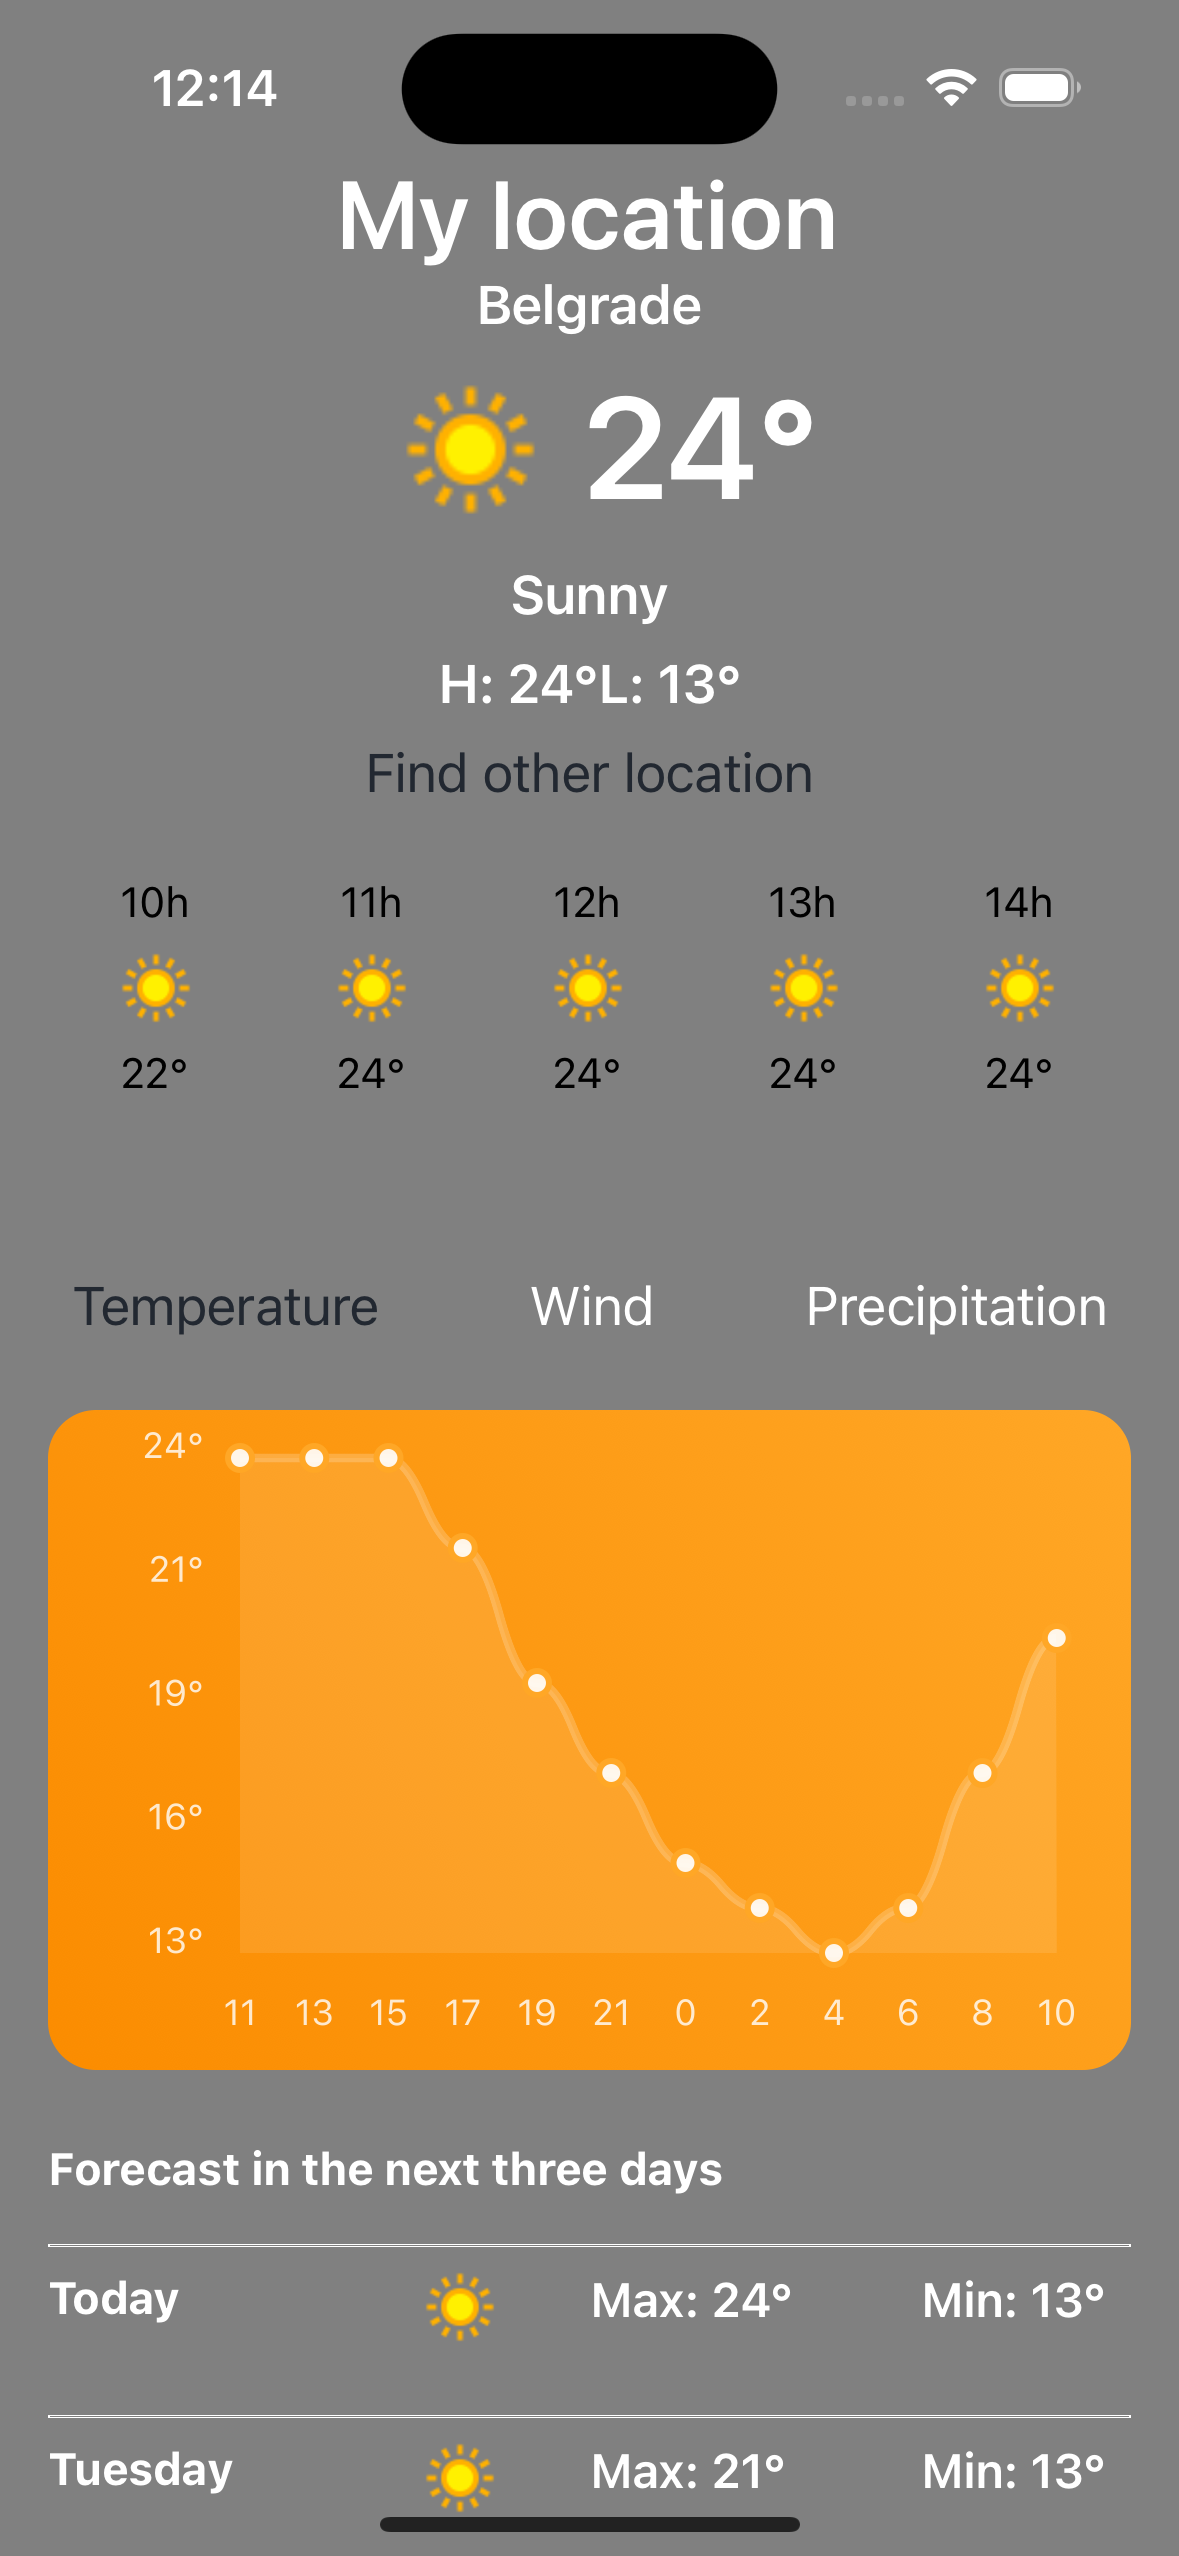
\includegraphics[width=5cm]{docs/images/chapterFour/mainScreen.png} }}%
    \qquad
    \subfloat[\centering Ekran za pretragu destinacije]{{
\includegraphics[width=5cm]{docs/images/chapterFour/searchScreen.png} }}%
\end{figure}

\newpage
\subsection{Ekran za vremensku prognozu}

Glavni ekran aplikacije predstavlja ekran sa svim parametrima vremenske prognoze. Sastoji se od pet sekcija. U nastavku ćemo analizirati svaku.

\begin{enumerate}
    \item Prva sekcija predstavlja podatke o trenutnoj lokaciji i temperaturi. Takođe, tu imamo podatke u maksimalnoj i minimalnoj dnevnoj temperaturi kao i o tome kakvo je vreme napolju.
    \item Nakon ovoga nalazi se dugme koje nas navigira na ekran za pretragu drugih destinacija na kojima želimo da vidimo vremensku prognozu.
    \item Zatim, imamo listu koja prikazuje temperature na datoj lokaciji u naredna dvadeset četiri časa. U pitanju je horizontalna, skrolabilna optimizovana lista. U kasnijim poglavljima ćemo dodatno govoriti o ovim optimizacijama.
    \item Ispod se nalazi komponenta koja prikazuje grafike kretanja određenih parametara kroz vreme. Posmatra se period od dvadeset četiri časa i korisnik je u mogućnosti da selektuje parametar koji ga interesuje.
    \item Na kraju, imamo sekciju koja predstavlja vremensku prognozu za naredne dane. Realizovana je takođe kao optimizovana lista, sa izmenom da je sada vertikalna lista u pitanju.
\end{enumerate}

\subsection{Ekran za pretragu destinacije}

Drugi ekran u našoj aplikaciji služi za pretragu destinacije na kojoj korisnik želi da pogleda vremensku prognozu. Što se tiče korisničkog interfejsa na ovom ekranu, možemo videti da je malo jednostavniji u odnosu na prvi ekran. Kao što vidimo sa slike, izdvajaju se dve glavne celine.

\begin{enumerate}
    \item Na samom vrhu ekrana nalazi se navigacijsko zaglavlje koje je izmenjeno tako da bude komponenta za unos teksta. Ovde korisnik preko tastature unosi željenu lokaciju i preko aplikacijskog programskog interfejsa (eng. Application Programming Interface - API) dohvatamo niz lokacija za uneti teskt.
    \item Uloga druge sekcije jeste da se prikažu podaci koje nam je API vratio. Realizovana je takođe kao optimizovana lista.
\end{enumerate}

\subsection{WeatherAPI}

U svrhe dohvatanja podataka potrebnih za izradu ove aplikacije korišćen je WeatherAPI. U pitanju je API koji nam daje nekoliko krajnjih tačaka (eng. endpoint). Konkretno, mi smo koristili dva. 

\begin{enumerate}
    \item Forecast API - ovaj API nam služi za dohvatanje podataka o vremenskoj prognozi. Odgovor servera sastoji se iz tri celine. Podaci o trenutnoj lokaciji, podaci o trenutnom vremenu i podaci o vremenskoj prognozi za naredne dane.
    \item Search API - uloga ove krajnje tačke jeste da nam vrati sve lokacije koje počinju nekim prefiksom koji je korisnik uneo. 
\end{enumerate}

\newpage

\begin{figure}[h]
    \centering
    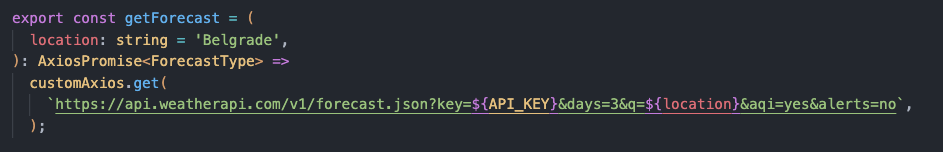
\includegraphics[scale=0.5]{docs/images/chapterFour/forecastAPI.png}
    \caption{API za vremensku prognozu}
    \label{fig:forecastAPI}
\end{figure}

\chapter{Sistem za merenje performansi aplikacije}

U savremenom razvoju softvera, efikasnost i performanse jedan su od ključnih aspekata za uspeh na tržištu. Uspeh naše aplikacije direktno zavisi od zadovoljstva korisnika, a to zadovoljstvo nemoguće je postići ukoliko aplikacija nije performantna. Ovo jeste razlog za razmatranje i uvođenje sistema za merenje performansi koji nam može pružiti jasnu sliku o ponašanju aplikacije u različitim uslovima. 
\newline
U ovom poglavlju upoznaćemo se sa različitim sistemima za merenje performansi i detaljnije se zadržati na sistemu Sentry. Proćićemo neophodne korake za integraciju ovog sistema u našu aplikaciju, a zatim se upoznati sa svime što nam isti pruža. Takođe, bavićemo se optimizovanim listama kao jedinom od ključnih koncepata u razvoju mobilne aplikacije.

\section{Alati za merenje performansi}

Kao što smo prethodno naveli, postoji veliki broj dostupnih platformi koje nam omogućavaju da integrišemo merenje performansi u našu aplikaciju. Pre nego što se upustimo u taj korak neophodno je upoznati se sa svima i odlučiti koji od tih alata najviše odgovara našim potrebama. U nastavku ove sekcije upoznaćemo se sa nekoliko najpopularnijih alata.

\subsection{React Native Performance Monitor}

React Native Performance Monitor je ugrađeni alat koji dolazi u okviru React native radnog okvira. On nam pruža osnovne informacije o performansama koje uključuju:

\begin{enumerate}
    \item Praćenje broja frejmova u sekundi (eng. Frame Per Second - FPS) - možemo pratiti dva seta FPS metrika. Jedan jeste za JavaScript nit, dok je drugi za glavnu, odnosno nit korisničkog interfejsa. Ovo nam omogućava da u realnom vremenu pratimo ove metrike i identifikujemo zbog čega dolazi do para performansi u nekom određenom momentu. Optimalno je da obe ove metrike budu blizu 60 FPS.
    \item Upotreba memorije - druga metrika koju možemo pratiti jeste količina radne memorije koju aplikacija koristi. Ovo nam je idealno za pronalaženje curenja memorije ili drugih problema vezanih za upravljanje memorijom.
\end{enumerate}

\begin{figure}[h]
    \centering
    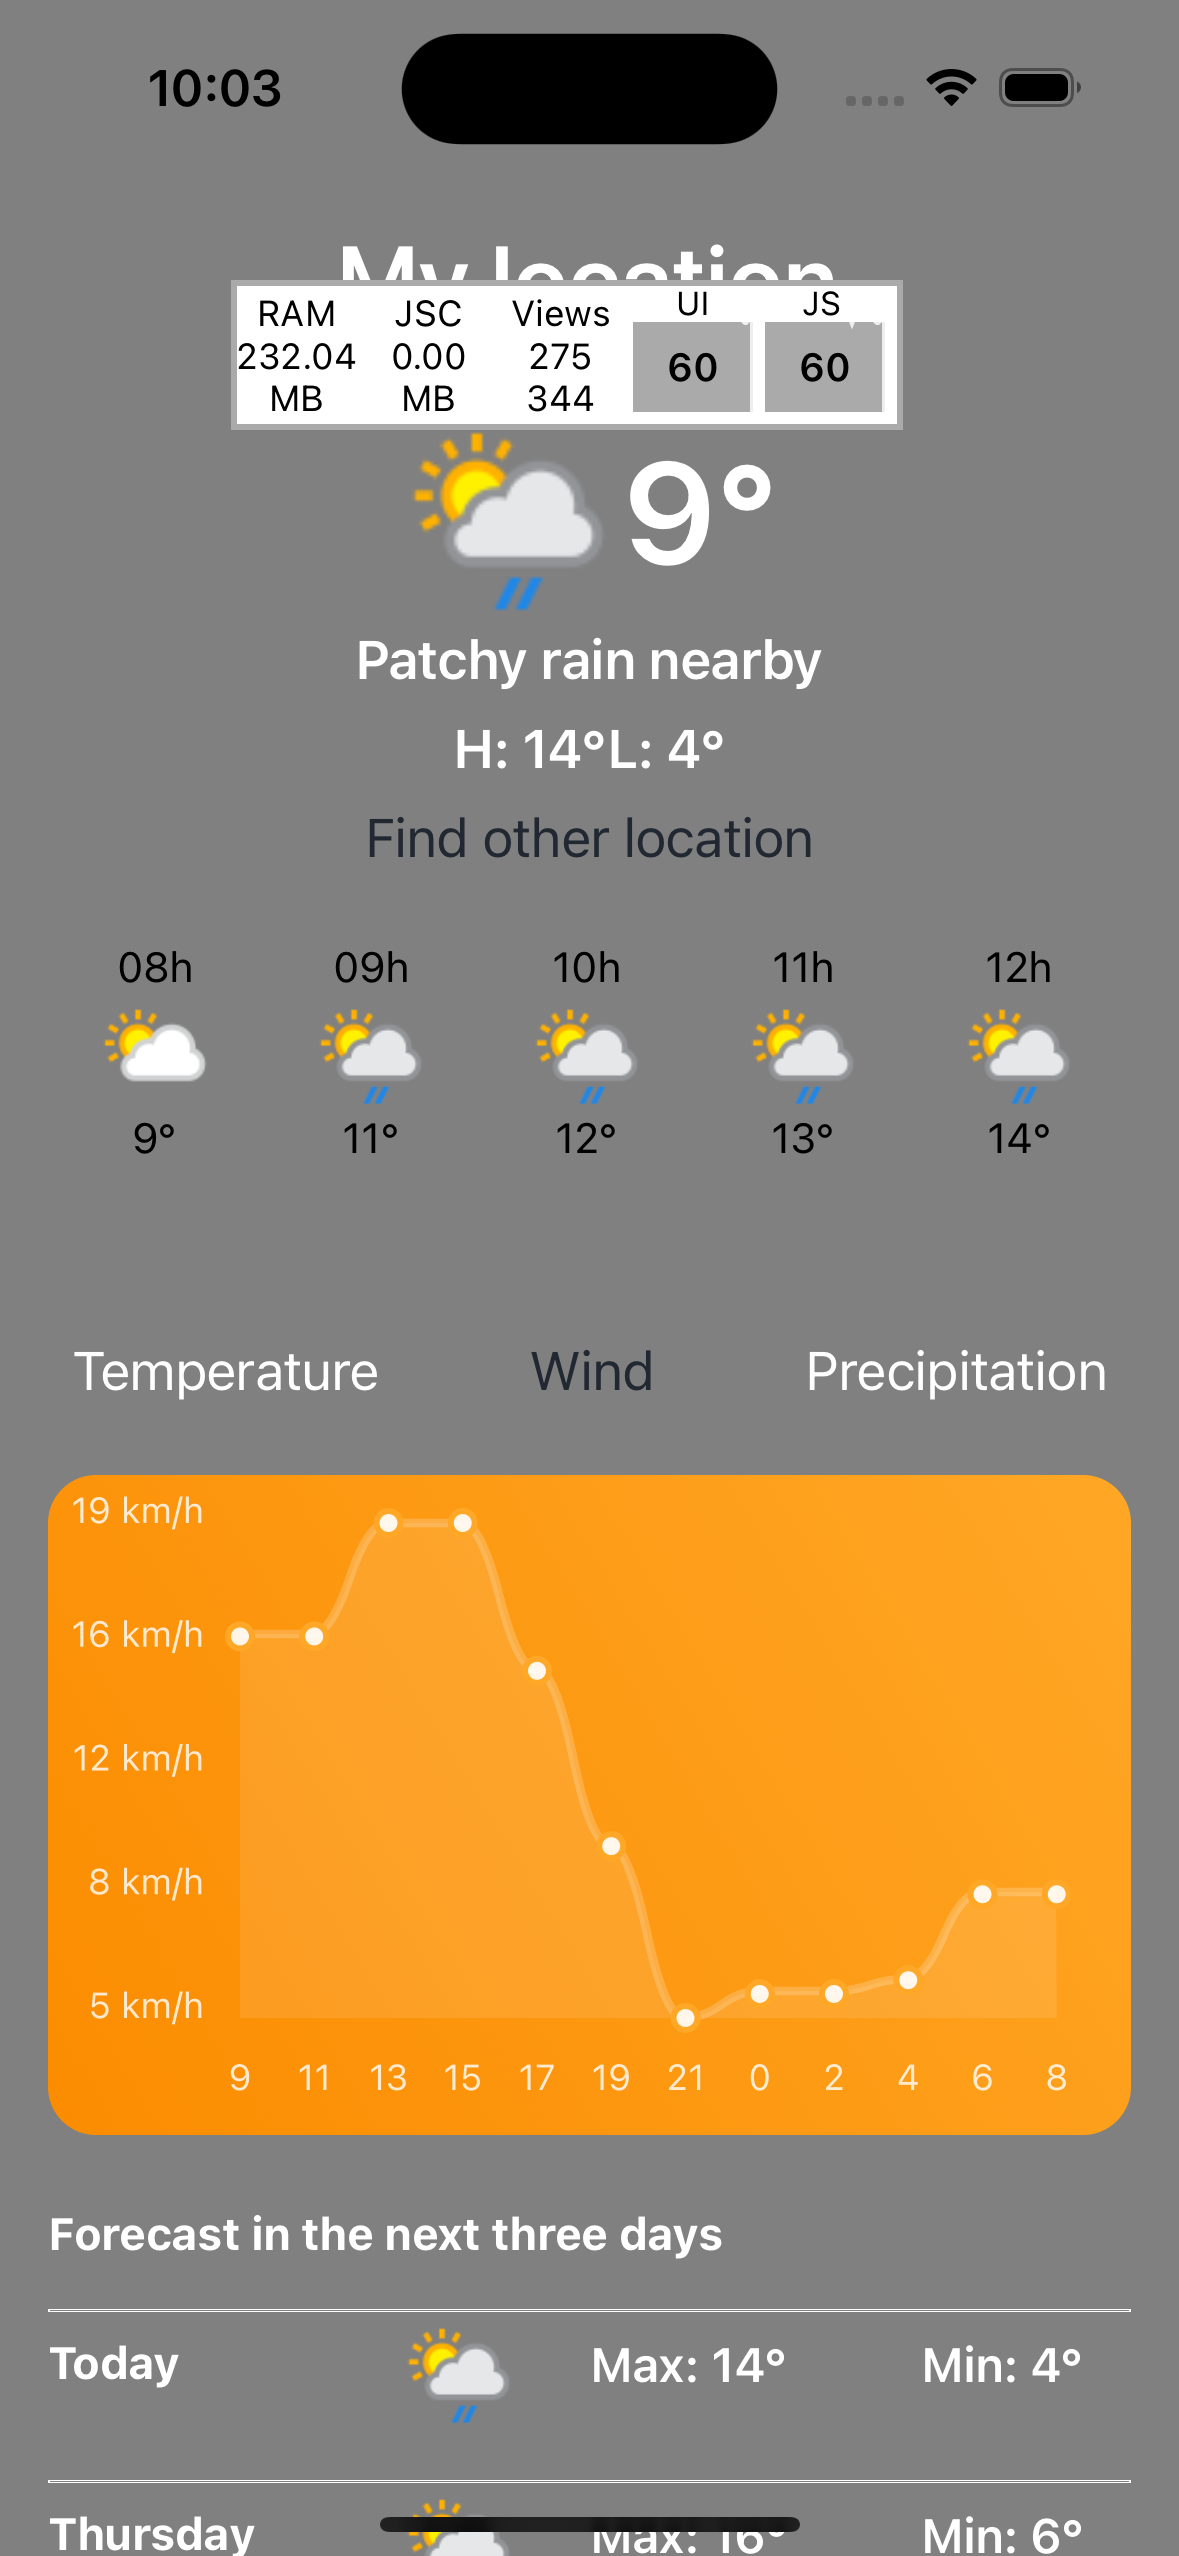
\includegraphics[scale=0.1]{docs/images/chapterFive/reactNativePerfMonitor.png}
    \caption{React Native Performance Monitor}
    \label{fig:reactNativePerformanceMonitor}
\end{figure}

Iako je React Native Performance Monitor koristan za osnovno praćenje performansi aplikacije, on nije dovoljno detaljan i ne pruža nam dublji uvid u performanse aplikacije.

\subsection{Fliper}

Fliper (eng. Flipper) je platforma za debagovanje koja je posebno dizajnirana za mobilne aplikacije, uključujući one razvijene pomoću React Native radnog okvira. Jedan od ključnih dodataka unutar Flipera jeste \textit{performance monitoring} dodatak koji omogućava programerima detaljan uvid u performanse aplikacije. Ovaj dodatak pruža kompletan set alata za analizu kako se aplikacija ponaša u realnom vremenu, omogućavajući programerima da identifikuju sporije delove aplikacije, analiziraju upotrebu resursa i dijagnostikuju probleme koji utiču na performanse. Uz mogućnost vizualnog prikaza performansi, kao što su FPS (eng. Frame Per Second) grafici i merni podaci o memoriji, Fliper nudi jednostavan i intuitivan interfejs za praćenje ključnih performansi aplikacije. Takođe, alat podržava razne dodatke koji se mogu lako integrisati i koristiti za specifične potrebe projekta, što Fliper čini nezamenjivim alatom u arsenalu modernih mobilnih developera.

\begin{figure}[!h]
    \centering
    \subfloat[\centering Osnovne metrike]{{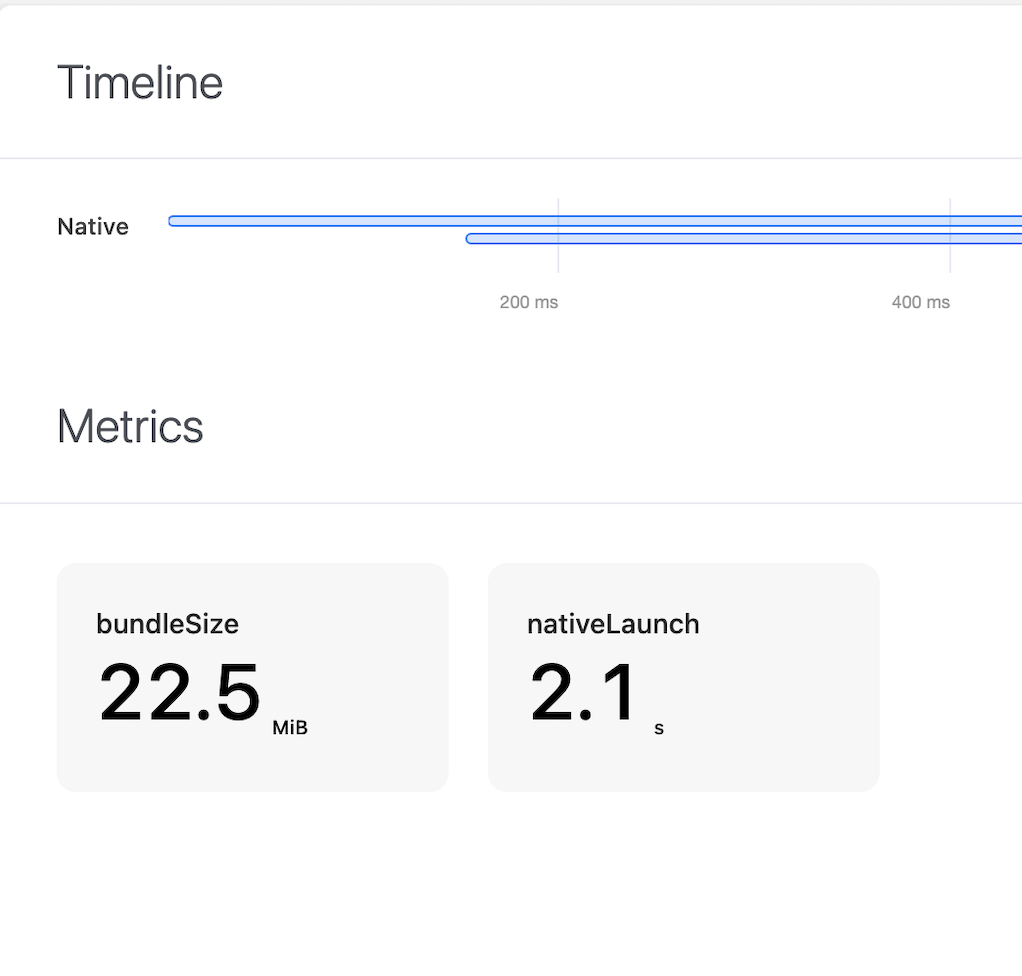
\includegraphics[width=5cm]{docs/images/chapterFive/flipperBasic.png} }}%
    \qquad
    \subfloat[\centering Merenje FPS-a]{{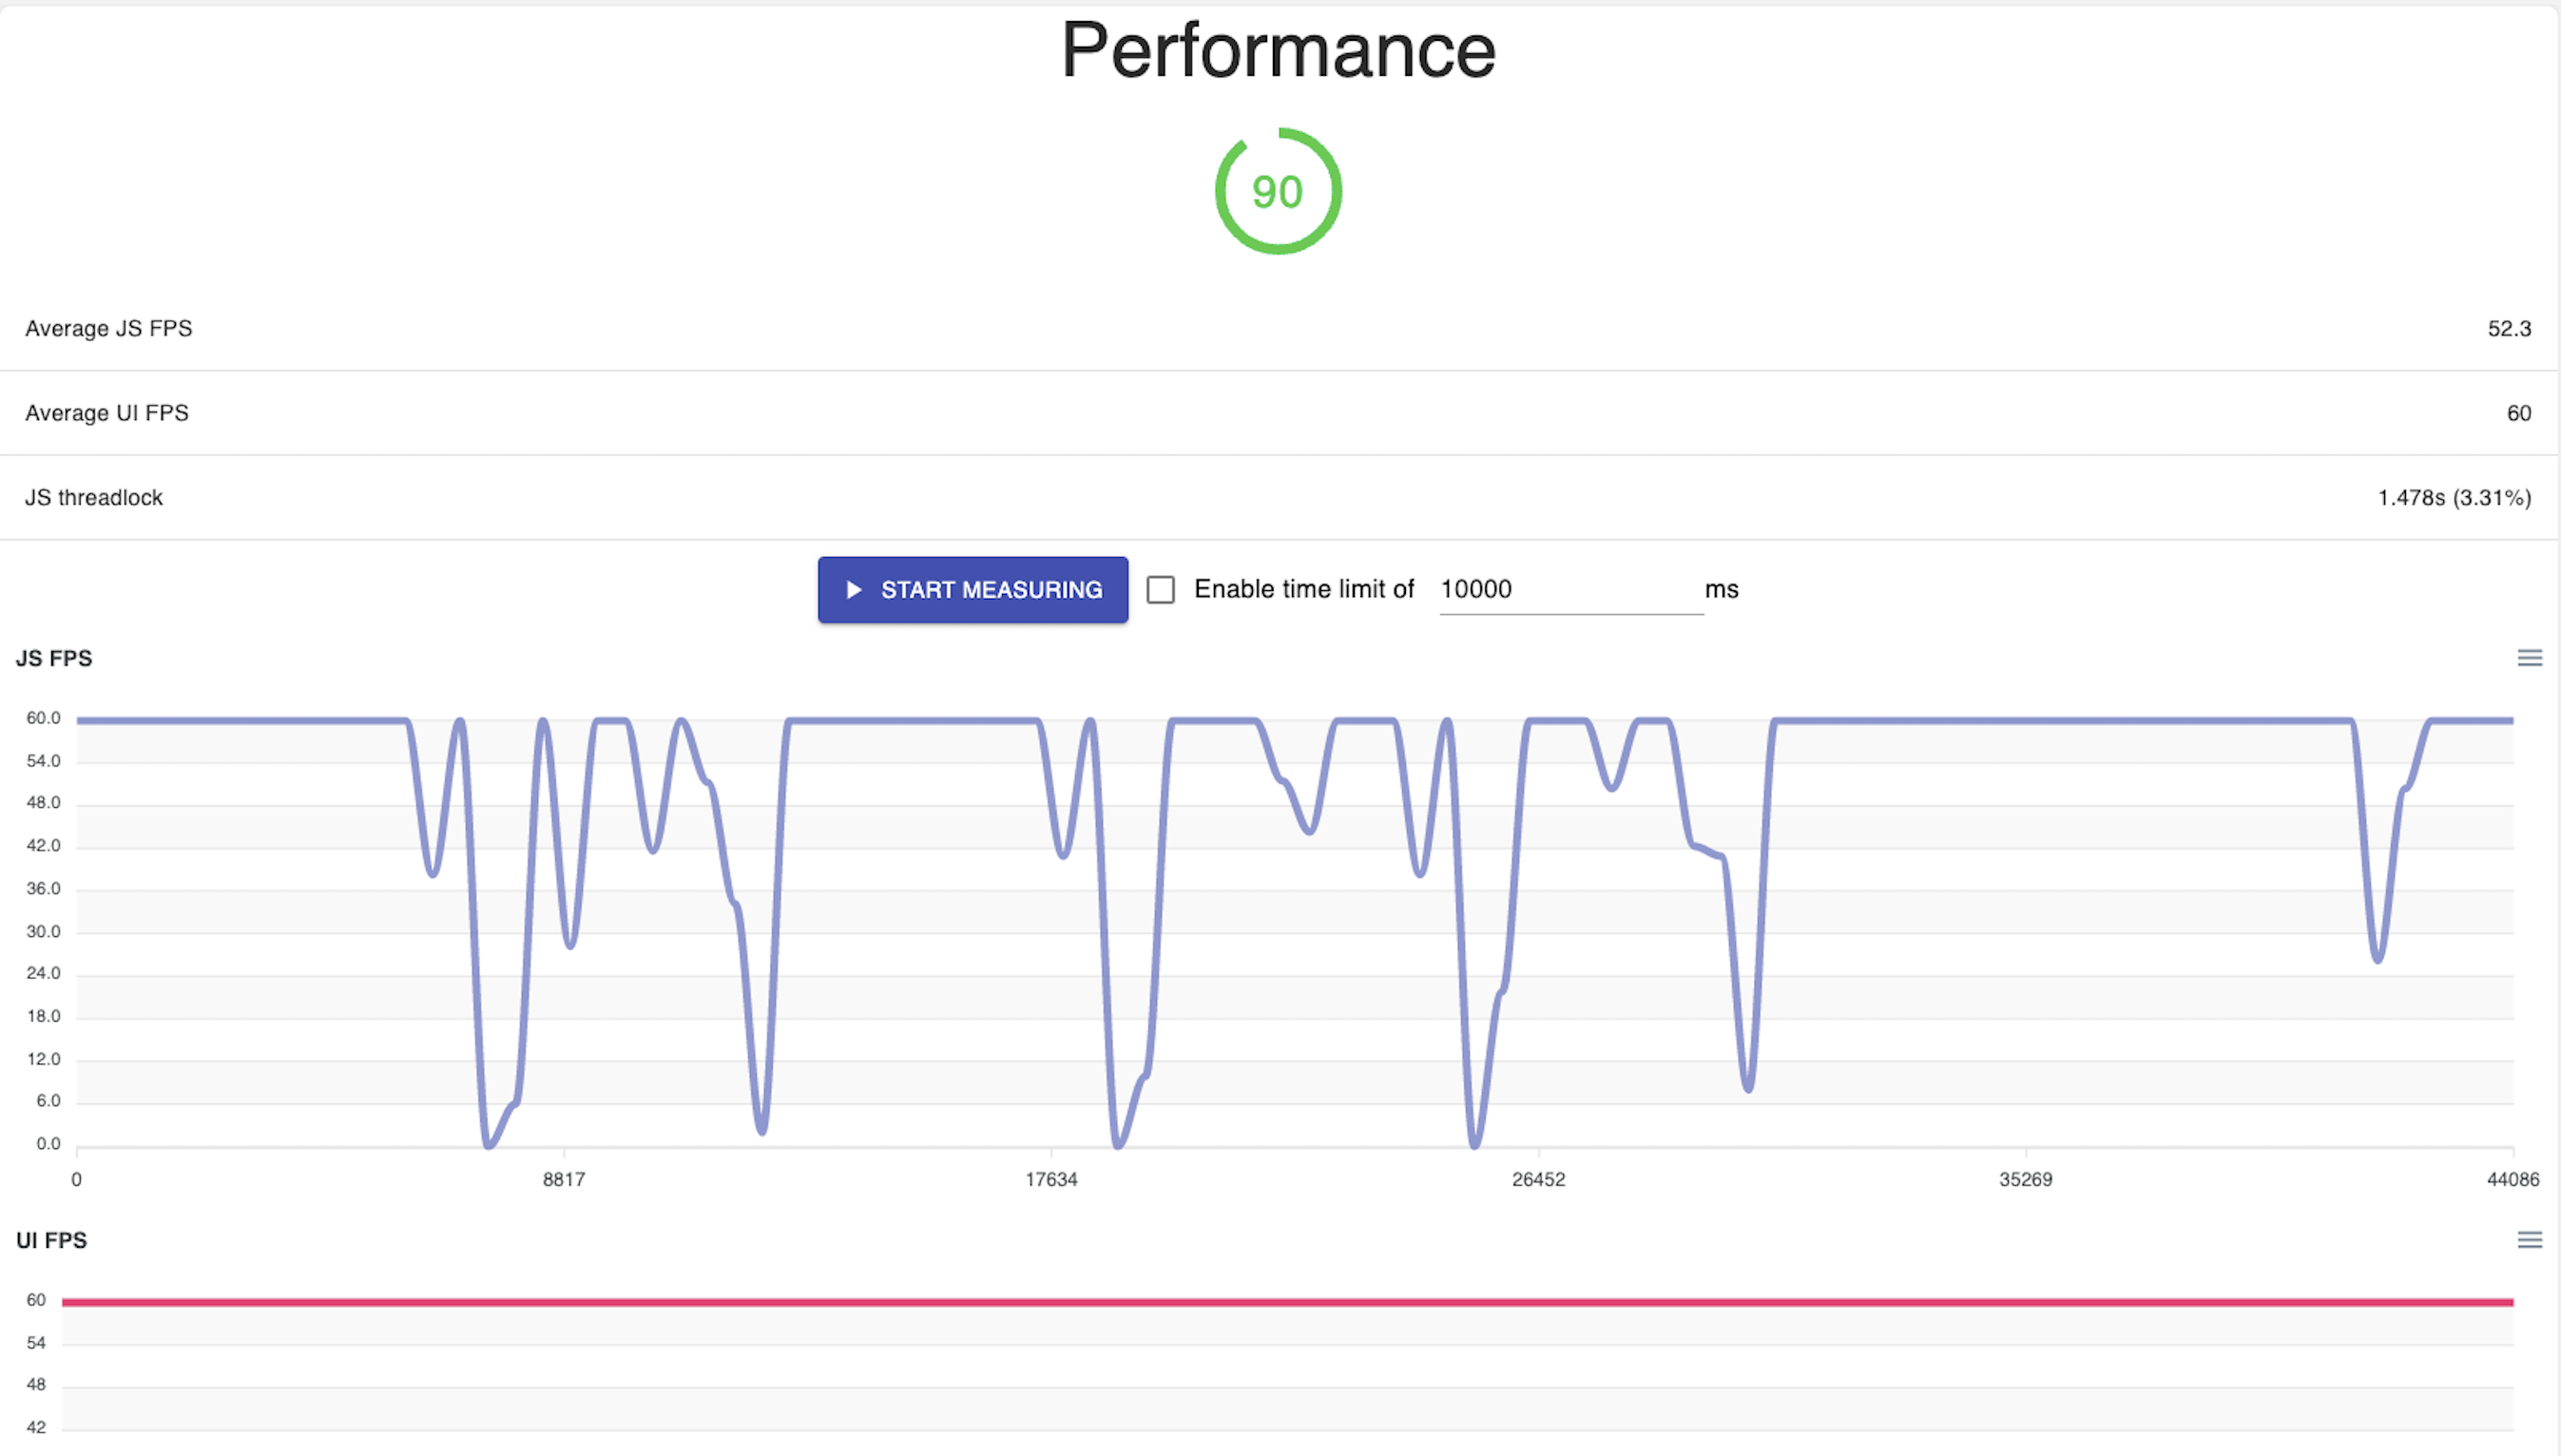
\includegraphics[width=5cm]{docs/images/chapterFive/fliperPerf.png} }}%
\end{figure}

\section{Sentry}

U ovoj sekciji detaljno ćemo se upoznati sa alatom Sentry. On predstavlja veoma snažan alat za nadgledanje grešaka i merenje performansi i veoma je popularan među programerima koji se bave optimizacijom i održavanjem zdravlja aplikacije u realnom vremenu. U kontekstu merenja performansi mobilnih aplikacija, Sentry nudi napredne funkcionalnosti koje programerima omogućavaju da precizno detektuju i analiziraju izvore problema koji utiču na korisničko iskustvo. Ovaj alat ne samo da automatski hvata greške unutar aplikacije, već pruža i detaljne uvide u performanse aplikacija, beležeći vremena odziva, broj grešaka i kroz analizu transakcija omogućava duboko razumevanje performansi aplikacije. Pomoću ovog alata, timovi mogu brzo reagovati na probleme, optimizovati aplikacije i značajno poboljšati stabilnost i brzinu aplikacija.

\subsection{Intregracija sistema Sentry}

Prvi korak ka korišćenju ovog sistema jeste integracija istog u našu aplikaciju. Ovaj korak je vrlo jednostavan i detaljno je objašnjen u dokumentaciji samog servisa. Za sam početak, neophodno je da se instalira biblioteka preko paketnog menadžera (eng. package manager). Nakon instalacije, potrebno je konfigurisati Sentry u glavnom fajlu aplikacije, gde se inicijalizuje Sentry sa odgovarajućim DSN (eng. Data Source Name) koji povezuje aplikaciju sa Sentry projektnim okruženjem. Ova konfiguracija omogućava Sentry-ju da automatski hvata izuzetke i greške u aplikaciji, kao i da pruža opcionalne funkcionalnosti poput ručnog slanja izveštaja o greškama, praćenje performansi i analizu korisničkih sesija. Unutar same konfiguracije bitno je podesiti procenat transakcija koje želimo da prosleđujemo na Sentry. Ovo se postiže uzorkovanjem i koristi se opcija \textit{tracesSampleRate} koja uzima vrednosti od 0 do 1. Drugi bitan parametar konfiguracije jesu sve integracije koje su nam potrebne. Ovo predstavlja vezu između biblioteka koje koristimo u aplikaciji i Sentry alata. Na primer, u našoj aplikaciji je potrebno da se doda integracija za navigacione transakcije kako bi Sentry znao kako da obradi iste.

\begin{figure}[h]
    \centering
    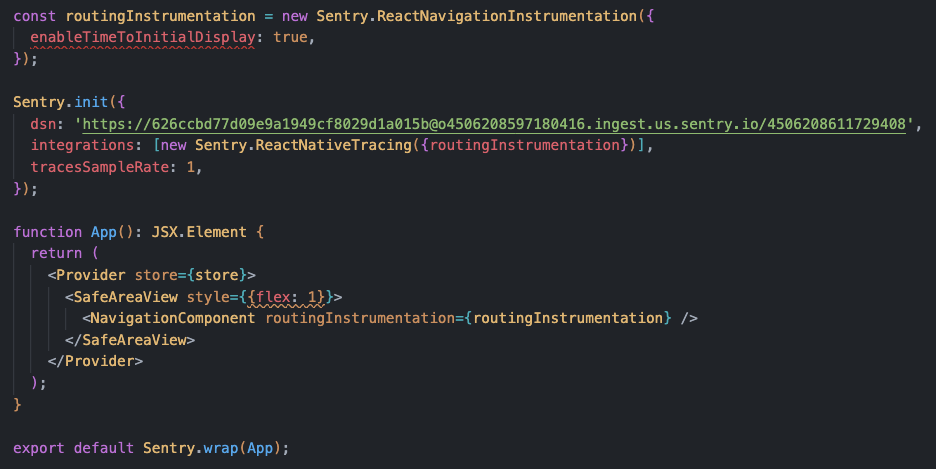
\includegraphics[scale=0.5]{docs/images/chapterFive/sentryIntegration.png}
    \caption{Sentry integracija u kodu}
    \label{fig:sentryIntegration}
\end{figure}

\subsection{Metrike alata Sentry za merenje performansi aplikacije}

Kada smo uspesno odradili integraciju alata Sentry sa našom aplikacijom, vreme je da pogledamo šta sve imamo na raspolaganju. Ekran koji ćemo videti kada u okviru alata Sentry navigiramo na odeljak za performanse izgleda kao na slici u nastavku.

\begin{figure}[h]
    \centering
    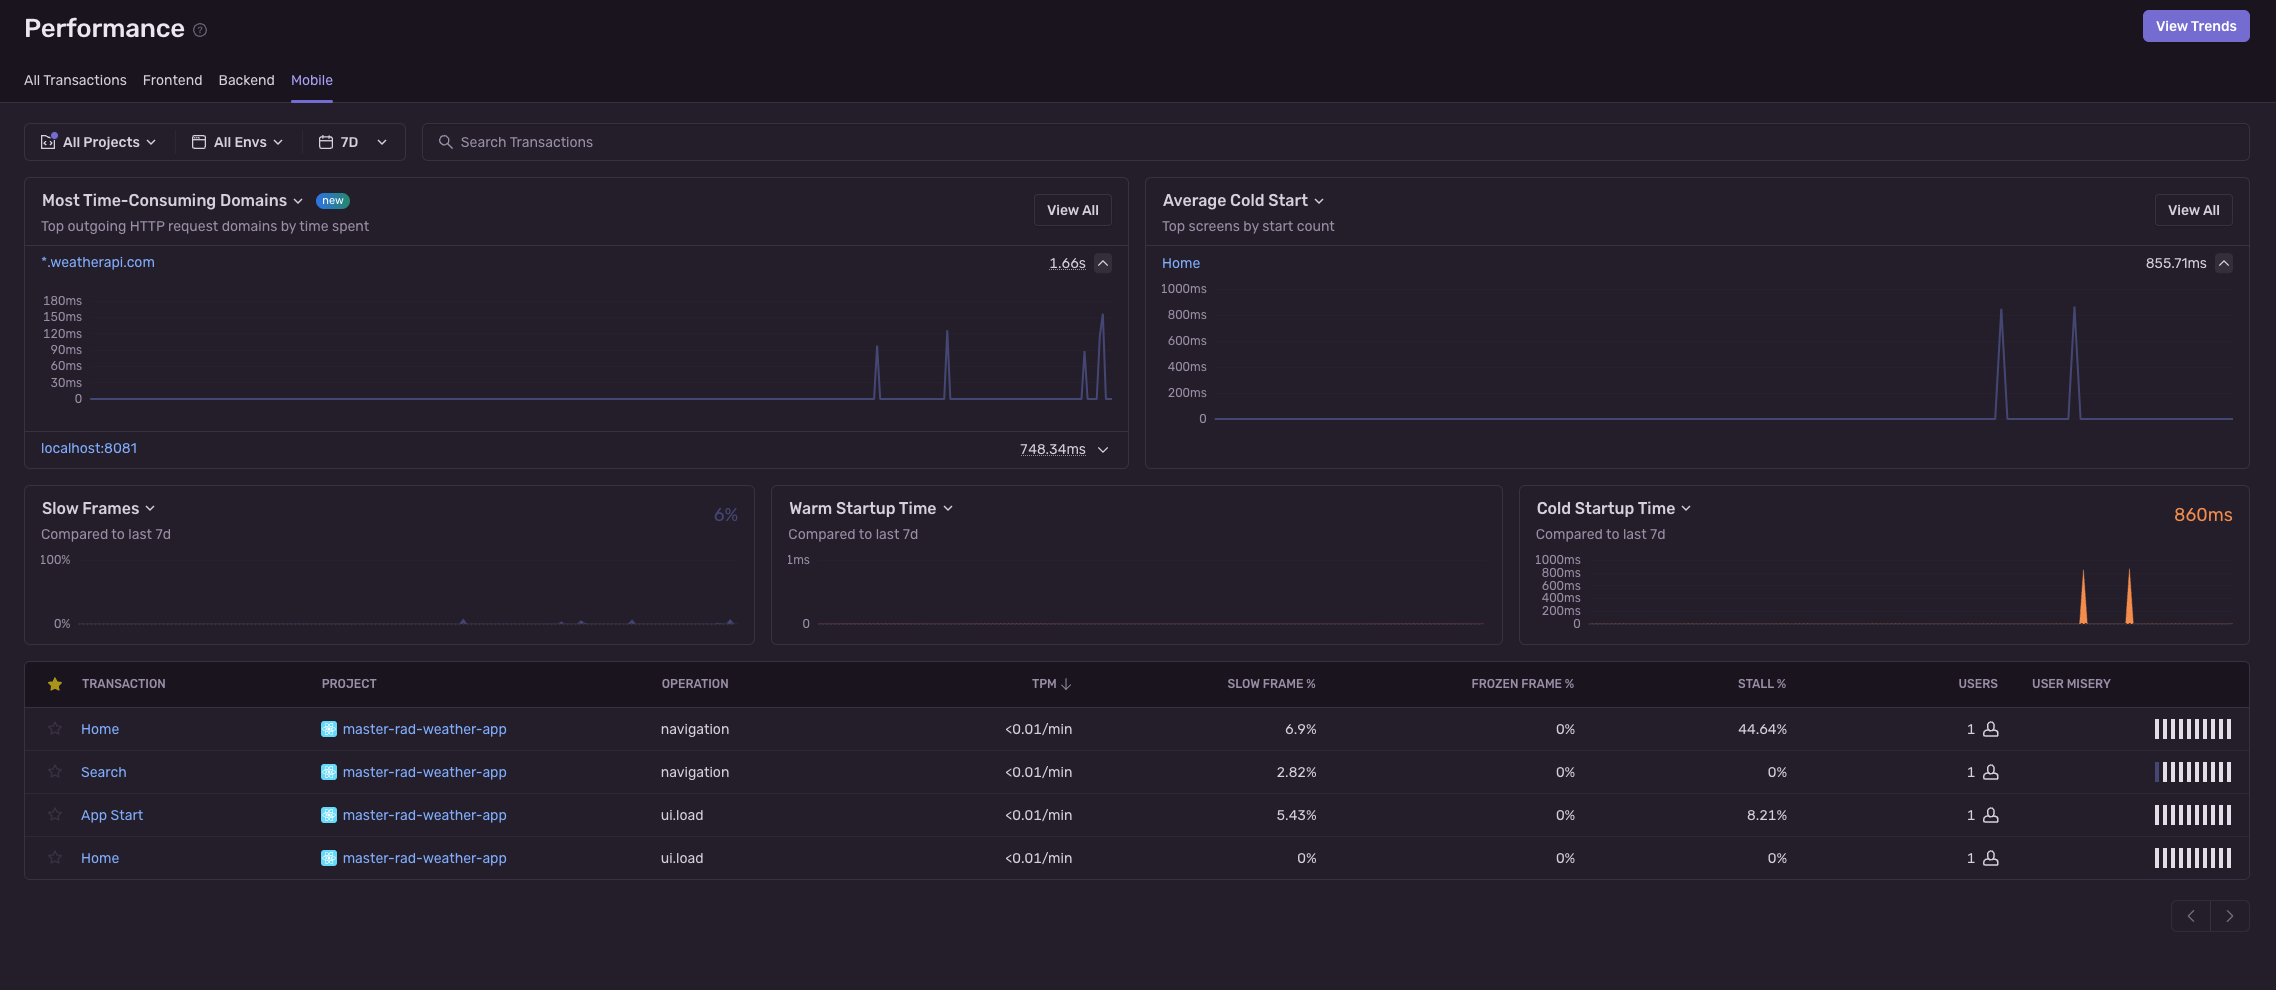
\includegraphics[scale=0.2]{docs/images/chapterFive/sentryPerfMetrics.png}
    \caption{Metrike za performanse koje nam pruža alat Sentry}
    \label{fig:sentryMetrics}
\end{figure}

Sada ćemo da analiziramo dostupne metrike i da vidimo šta one u stvari predstavljaju.

\begin{enumerate}
    \item Vreme inicijalnog pokretanja (eng. Cold Startup time) - jedna od primarnih performansnih metrika u razvoju mobilnih aplikacije jeste vreme inicialnog pokretanja. Ova metrika meri vreme potrebno da se aplikacija pokrene i postane potpuno funkcionalna nakon što je korisnik pokrenuo aplikaciju s potpuno neaktivnog ili "hladnog" stanja, odnosno kada aplikacija nije u memoriji uređaja. Ovo uključuje vreme potrebno za učitavanje aplikacije u memoriju, inicijalizaciju aplikacije, učitavanje početnih resursa i prikaz prvog ekrana korisniku. Brže vreme pokretanja može značajno poboljšati percepciju aplikacije od strane korisnika, smanjujući frustraciju i povećavajući zadovoljstvo. Pored samog korisničkog iskustva, ova metrika se u praksi koristi i za definisanje uskih grla prilikom pokretanja aplikacije. Često se tu dovlače resursi i vrše kalkulacije koje nisu potrebne za samo pokretanje aplikacije i neophodno ih je odložiti za kasnije. Kao referentna vrednost za produkcijske verzije aplikacija uzima se 400ms.
    \item Vreme reaktiviranja aplikacije (eng. Warm startup time) - ova metrika predstavlja vreme da se aplikacija reaktivira i postane potpuno funkcionalna iz tzv. "toplog" stanja, kada je aplikacija već delimično učitana u memoriji uređaja, ali nije aktivna. Ovo može uključiti situacije kada je aplikacija minimizirana ili kada korisnik prebacuje između aplikacija. Ova metrika time se fokusira na brzinu kojom aplikacija može ponovo postati aktivna i spremna za interakciju, što je ključni faktor za korisničko iskustvo, posebno u situacijama kada korisnici očekuju brz odgovor aplikacije nakon prekida korišćenja. Praćenje i optimizacija ove metrike su važni za poboljšanje fluidnosti i responzivnosti aplikacije, što može značajno uticati na zadovoljstvo korisnika i percepciju performansi aplikacije. Developeri koriste ovu metriku za identifikaciju problema u upravljanju resursima ili kodnim blokovima koji mogu usporiti reaktivaciju aplikacije, te rade na njihovom otklanjanju kako bi optimizovali ukupno korisničko iskustvo.
    \item Spori kadrovi (eng. Slow frames) - dobre performanse aplikacijese često poistovećuju sa fluidnim radom iste. To se, pored posmatranja golim okom, može izmeriti i jedna od metrika koja se koristi za to jeste broj sporih kadrova. Odnosi se na broj kadrova (eng. frames) u animacijama ili prikazivanju sadržaja na ekranu koji se ne izvršavaju u optimalnom vremenskom intervalu, što dovodi do zaostajanja (eng. lagging) i seckanja (eng. stuttering). Tipično, aplikacije bi trebalo da održavaju stopu od 60 sličica po sekundi (eng. fps) za glatko i prirodno korisničko iskustvo. Kadrovi koji se izvršavaju sporije od ove stope klasifikuju se kao "spori". Ova metrika je ključna za razvojne timove kako bi razumeli kako njihova aplikacija performira u stvarnim uslovima korišćenja, posebno kada su u pitanju zahtevnije operacije kao što su animacije, skrolovanje ili tranzicije između ekrana. Praćenje sporih kadrova omogućava programerima da identifikuju i optimizuju delove aplikacije koji narušavaju fluidnost, tako što prilagođavaju animacije, optimizuju renderovanje komponenti ili redukuju opterećenje procesora i grafičkog procesora.
    \item Zamrznuti kadrovi (eng. Frozen frames) - ova metrika odnosi se na period kada aplikacija ne reaguje i ne osvežava svoj prikaz, što rezultira zaustavljanjem interaktivnosti i vizuelnog prikaza na korisničkom interfejsu. Ova pojava se obično dešava kada aplikacija naleti na teške ili blokirajuće operacije koje zaguše glavnu nit, čineći da aplikacija postane neoperativna za milisekunde ili čak sekunde. Takvi zamrznuti kadrovi mogu značajno narušiti korisničko iskustvo, jer korisnici očekuju brzu i glatku interakciju sa aplikacijama. Praćenje i analiziranje zamrznutih kadrova neophodno je za otkrivanje i razrešenje uzroka ovih performansnih problema. To uključuje identifikovanje i optimizaciju teških procesa koji opterećuju CPU (eng. Central Processing unit) ili preduzimanje koraka za asinhrono izvršavanje dugotrajnih zadataka. Time se osigurava da korisnički interfejs ostaje responzivan i prijatan za korišćenje, što je ključno za održavanje visokog nivoa zadovoljstva korisnika.
    \item Korisničko nezadovoljstvo (eng. User misery) - ovo je interna Sentry metrika. Predstavlja broj različitih korisnika koji su iskusili vreme učitavanje četiri puta veće od podešene granice na nivou projekta. 
\end{enumerate}

Kao što se vidi na slici, korisnički interfejs alata Sentry pruža nam potpunu mogućnost da postavljamo metrike koje su nama relevantne. Dakle, prilikom postavljanja sistema za praćenje performansi, razvojni tim mora da definiše metrike koje želi da prati i da ih postavi u samom alatu. Sentry podržava i kreiranje našim metrika ukoliko shvatimo da nam treba metrika koja nije podržana od strane samog alata. 

\subsection{Performanse ekrana}

Alat Sentry daje nam podršku i da pratimo performanse pojedinačnih ekrana u našoj aplikaciji.

\begin{figure}[h]
    \centering
    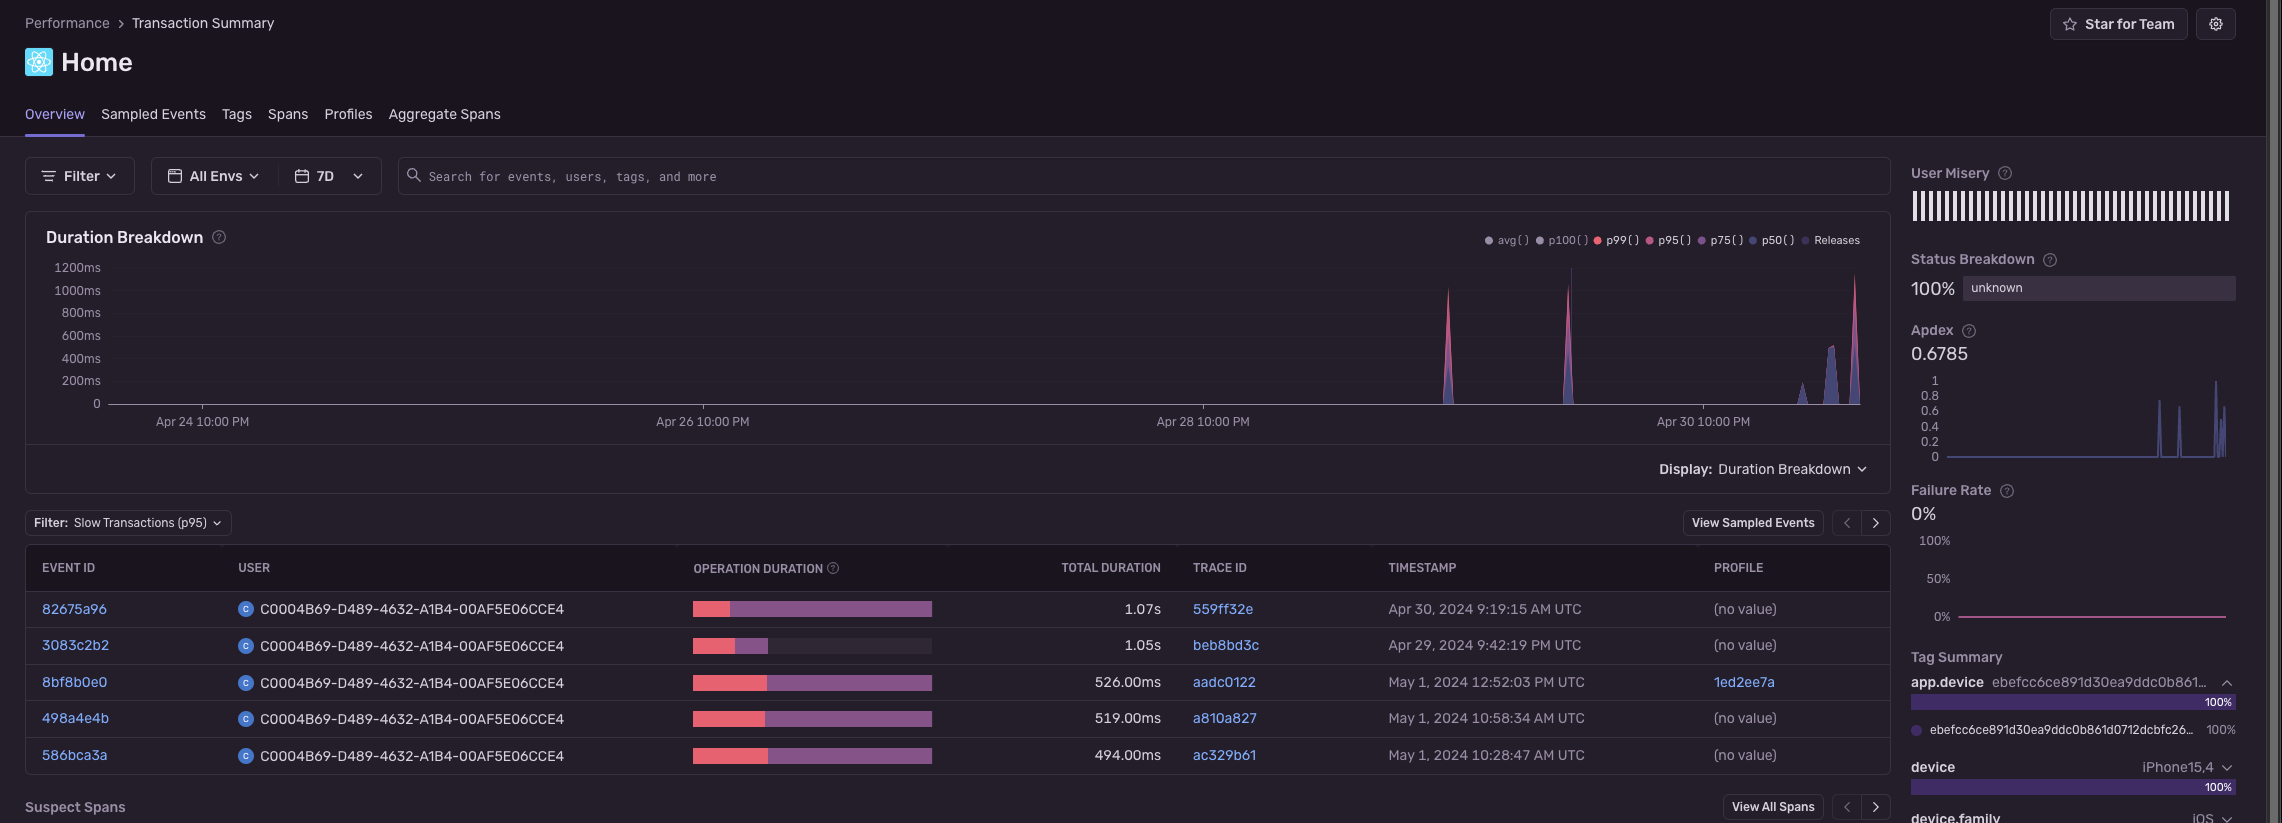
\includegraphics[scale=0.2]{docs/images/chapterFive/sentryHomeScreen.png}
    \caption{Metrike za glavni ekran aplikacije}
    \label{fig:mainScreenMetrics}
\end{figure}

Na prethodnoj slici vidimo da za svaki ekran imamo listu transakcija koje uključuju navigiranje na isti i učitavanje svih potrebnih podataka za prikaz. Sentry nam daje informacije o tome koliko je trajalo dohvatanje svih potrebnih podataka sa servera (prikazano narandžastom bojom), i trajanje renderovanja korisničkog interfejsa (prikazano ljubičastom bojom).

\subsection{Praćenje metrika}

Nakon što smo uspešno integrisali sistem za praćenje performansi i postavili sve metrike koje želimo da pratimo neophodno je postaviti sistem za obavestavanje. Naime, vrlo je nepraktično da neko konstantno proverava sve metrike koje se prate i da reaguje ukoliko naiđe na nešto problematično. Ovakav pristup zahtevao bi da neko konstantno prolazi i gleda metrike kao i da zna tačno kako iste treba da se ponašaju. Jasno je da je ovakav pristup dugoročno neodrživ. Sentry ovo prevazilazi konceptom obavestenja ili uzbune (eng. Alert). Naime, mi kao korisnik alata možemo da definišemo granicu kada je neka metrika na nezadovoljavajućem nivou i da kazemo alatu da ukoliko ista ikada padne ispod te granice da se podigne uzbuna i da nas obavesti o problemu. Na ovaj način bismo morali jednom da postavimo ove okidače i da reagujemo samo kada se podigne uzbuna. U međuvremenu, praktično bismo mogli da zaboravimo na ove metrike.

\begin{figure}
    \centering
    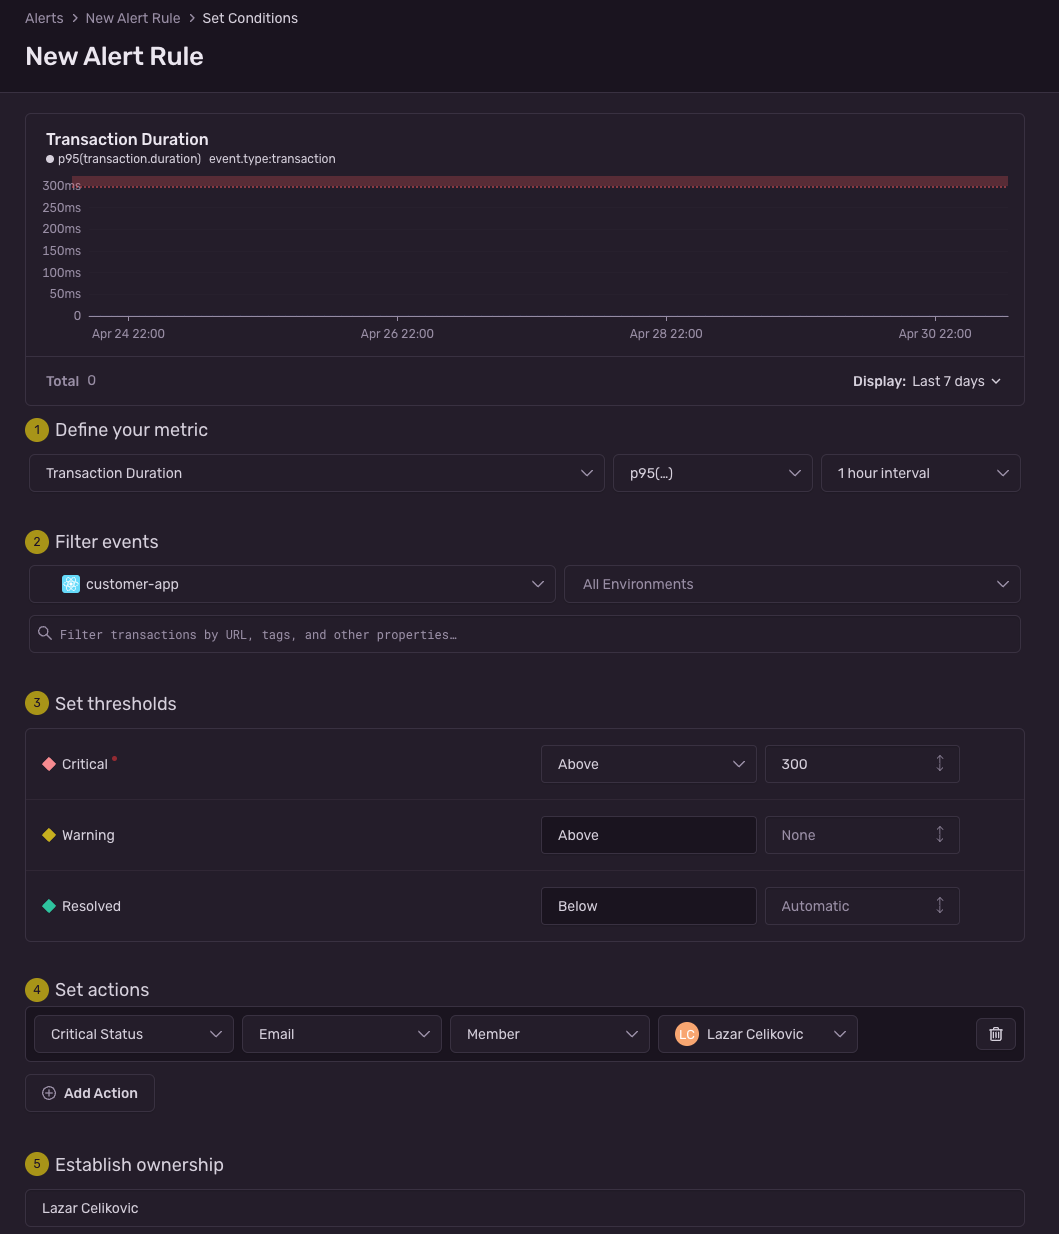
\includegraphics[scale=0.3]{docs/images/chapterFive/addRule.png}
    \caption{Dodavanje uzbune za metriku}
    \label{fig:addRuleForMetric}
\end{figure}

U konkretnom slučaju, dodali smo novu uzbunu za metriku \textit{Dužina trajanja transakcije}. U suštini, pravilo koje smo dodali glasi: "Ukoliko u intervalu od sat vremena, preko 95\% transakcija ima trajanje veće od 300ms okini uzbunu i obavesti korisnika putem mejla."

\section{Optimizacija listi za prikazivanje}

Liste su jedan od ključnih elementa u dizajnu mobilnih aplikacija, omogućavajući korisnicima efikasno i intuitivno pregledanje sadržaja. One služe kao ključna komponenta za organizovanje podataka u lako dostupan i razumljiv format, što je posebno važno u mobilnom okruženju gde je prostor ograničen i korisnička pažnja kratkotrajna. U programiranju mobilnih aplikacija, efektivna implementacija lista može značajno poboljšati korisničko iskustvo, pružajući brz pristup raznovrsnim informacijama. Bilo da se radi o listi kontakata, podešavanja ili kao u našem slučaju vremena po danima ili satima, liste omogućavaju korisnicima da lako navigiraju kroz aplikaciju i brzo pristupe željenim informacijama. Uz to, napredne tehnike poput lenjog učitavanja (eng. lazy loading) i beskonačnog skrolovanja (eng. infinite scrolling) mogu dalje optimizovati performanse i korisnički doživljaj, čineći liste još moćnijim alatom u arsenalu svakog programera mobilnih aplikacija.

\subsection{Komponenta FlatList i njeni problemi}

Komponenta FlatList u React Native radnom okviru je dizajnirana za efikasno prikazivanje dugačkih lista podataka, pružajući osnovne funkcionalnosti za upravljanje velikim količinama elemenata. Međutim, uprkos svojoj nameni, FlatList može susresti izazove sa performansama u određenim scenarijima. Problemi se najčešće javljaju kada lista sadrži složene elemente ili kada se učitava veliki broj podataka, što može dovesti do usporenja i povećane potrošnje memorije.

Kada svaki element liste zahteva intenzivno procesiranje ili ima kompleksne vizualne komponente, FlatList može doživeti pad performansi. Takođe, česti re-renderi izazvani promenama u stanju ili propovima koji se ne upravljaju pažljivo mogu dodatno opteretiti procesor i memoriju. Da bi se ovi problemi minimizovali, preporučuje se pažljiva optimizacija renderovanja elemenata, upotreba tehnika kao što su memoizacija za skuplje komponente, i efikasno upravljanje stanjem da se izbegnu nepotrebna ažuriranja. Implementacija paginacije (eng. windowing) gde se renderuju samo trenutno vidljivi elementi takođe može značajno poboljšati performanse FlatList komponente. Ovim pristupima osigurava se da FlatList ostane efikasan alat za upravljanje listama u aplikacijama koje razvijate koristeći React Native.

\begin{figure}[h!]
    \centering
    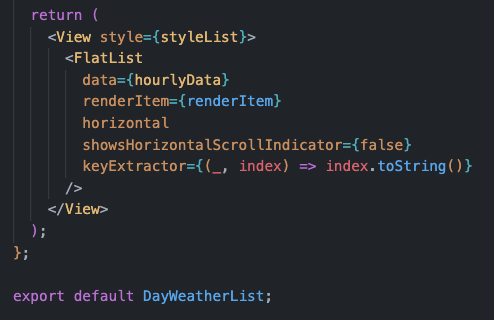
\includegraphics[scale=0.5]{docs/images/chapterFive/flatlistExample.png}
    \caption{Flatlist komponenta u kodu}
    \label{fig:flatListExample1}
\end{figure}

Sa slike iznad vidimo API FlatList komponente i možemo zaključiti da je isti veoma intuitivan. Naime, dva glavna polja jesu \textit{data} i \textit{renderItem}. Preko data polja prosleđujemo niz podataka našoj komponenti, dok preko polja renderItem govorimo na koji način treba da se prikaže svaki element tog niza. Polje keyExtractor nam služi kako bi listu optimizovali do neke mere, odnosno da svaki element liste ima svoj identifikator. Na ovaj način, komponenta razlikuje svaki pojedinačni element i pomoću tog znanja se odlučuje koje elemente treba ponovo renderovati kada dođe do promena u podacima.

\subsection{Prvi pokušaj rešavanja ovog problema}

Kako je problem sa performansama FlatList komponente bio prilično značajan, brzo je adresiran u krugovima programera mobilnih aplikacija. Kao rešenje ovog problema kreirana je RecyclerListView komponenta. Ona predstavlja komponentu veoma dobro optimizovanu za renderovanje ogromnog broja podataka. Inspirisana je RecyclerView komponentom na Androidu i UICollectionView na iOS operativnom sistemu. 


Ova komponenta je veoma performantna i bogata funkcionalnostima kao i ugrađena FlatList komponenta. Funkcioniše tako što se na pametan način vrši recikliranje komponenti koje su prethodno već renderovane i na taj način izbegava nepotrebno ponovno renderovanje. Ova tehnika poznata je kao reciklaža ćelija (eng. cell recycling) i dozvoljava nam da koristimo već renderovane komponente koje nisu više prisutne na ekranu za renderovanje novih.


Problem ove komponente jeste veoma neintuitivan API. Kao programer, morali ste potrošiti ogromnu količinu vremena da razumete kako sama komponenta radi da biste mogli da iskoristite prednosti koje ista pruža. Komponenta zahteva precizne predikcije za veličinu elemenata i ako iste nisu dobre performanse dosta padaju. Takođe, sav render se vrši na JavaScript niti što može dovesti na seckanja.

\subsection{FlashList biblioteka}

Rešenje problema pomenutih u prethodnim sekcijama ogleda se u biblioteci po imenu FlashList. Ona predstavlja performantnu alternativu za FlatList komponentu. Kao što smo rekli, FlatList komponenta nije imala zadovoljavajuće performanse, ali je bila laka za korišćenje, dok je RecyclerListView komponenta bila performantna, ali je njen API bio izrazito neintuitivan. Ideja biblioteke FlashList jeste da iskoristi najbolje iz oba pristupa i da kreira komponentu koja će biti veoma performanta, ali će zadržati API tako da korisnicima bude laka za korišćenje.


\begin{figure}[h!]
    \centering
    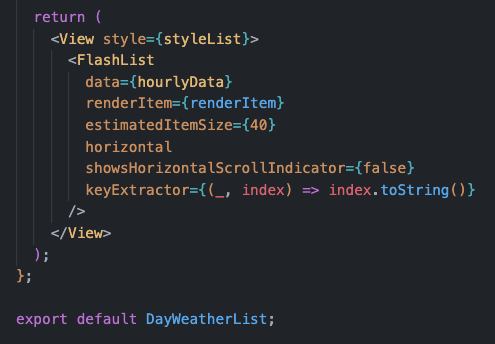
\includegraphics[scale=0.5]{docs/images/chapterFive/flashlistExample.png}
    \caption{Flashlist komponenta u kodu}
    \label{fig:flatListExample}
\end{figure}

Sa slike iznad vidimo kako izgleda korišćenje FlashList komponente u samom kodu. Prva stvar koju primećujemo jeste da je API skoro identičan sa FlatList komponentom. Jedina razlika jeste u estimatedItemSize polju koje je specifično za ovu biblioteku.


FlashList komponenta koristi estimatedItemSize polje kako bi odredila broj elemenata koji treba da budu prikazani na ekranu tokom inicijalnog renderovanja i prilikom skrolovanja. Kako sve ovo radi? Naime, umesto da se komponenta uništava kada neki element nestane sa ekrana, FlashList komponenta renderuje istu komponentu sa drugačijim parametrima. Prilikom korišćenja, bitno je da se ne koristi key polje u elementima liste jer će ovo sprečiti FlashList komponentu da radi recikliranje.


Na slikama ispod vidimo performanse prilikom korišćenja FlatList i FlashList komponenti. Možemo primetiti da je razlika u performansama drastična. Vidimo da prilikom korišćenja FlatList komponente imamo relativno često blokiranje JS niti, dok kod FlashList komponente to nije slučaj. Blokade se dešavaju na momente i to bas u momentu kada se dohvataju podaci sa backend servera (eng. Backend).

\begin{figure}[!h]
    \centering
    \subfloat[\centering FlatList performanse]{{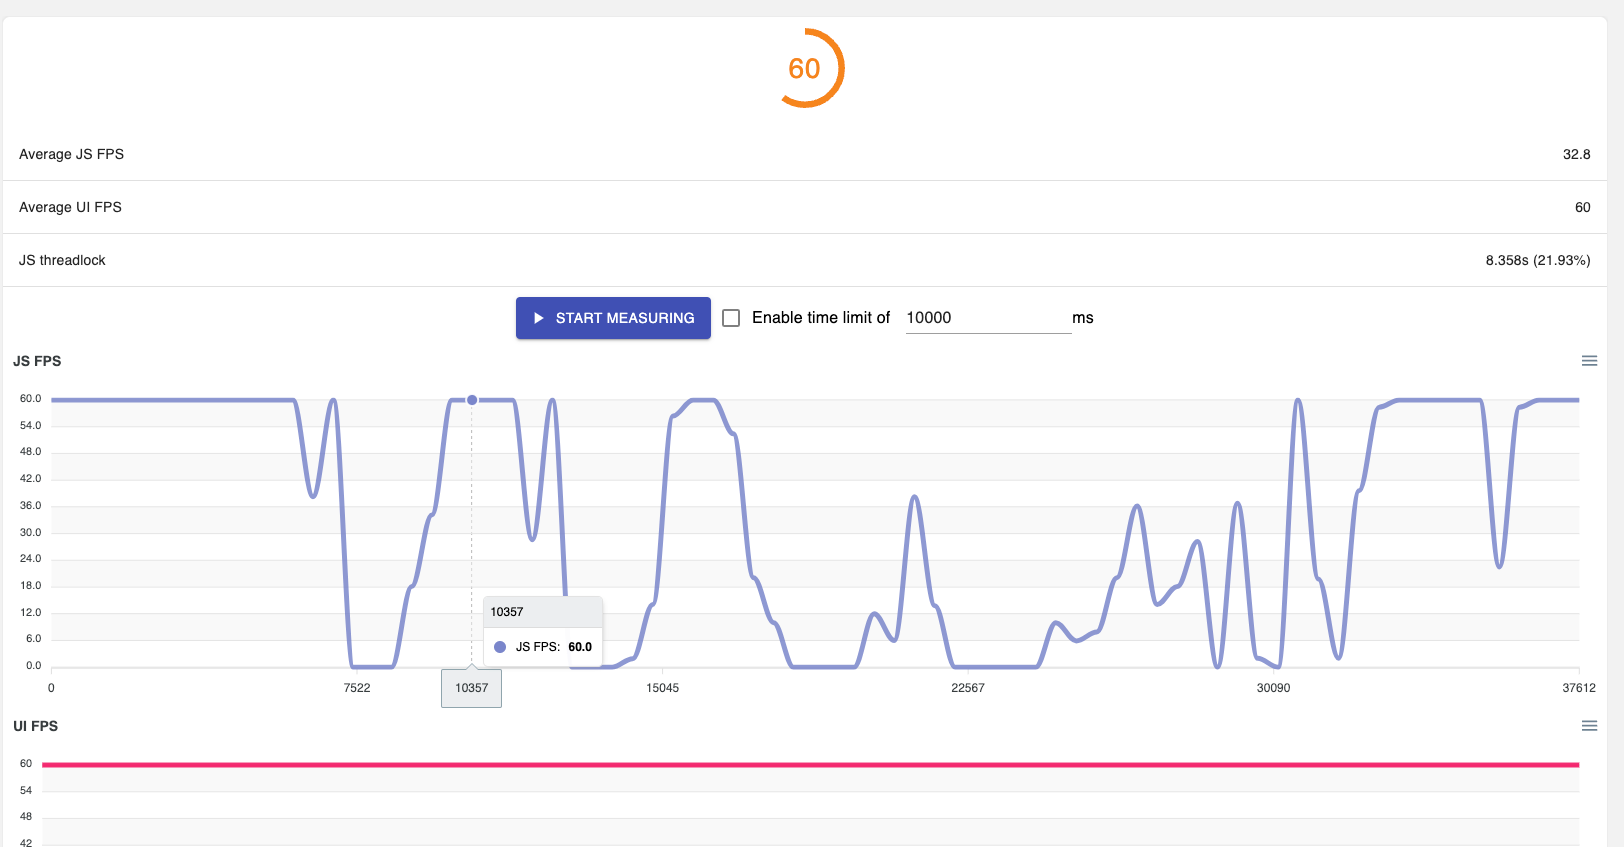
\includegraphics[width=6cm]{docs/images/chapterFive/flashListLowPerf.png} }}
    \qquad
    \subfloat[\centering FlashList performanse]{{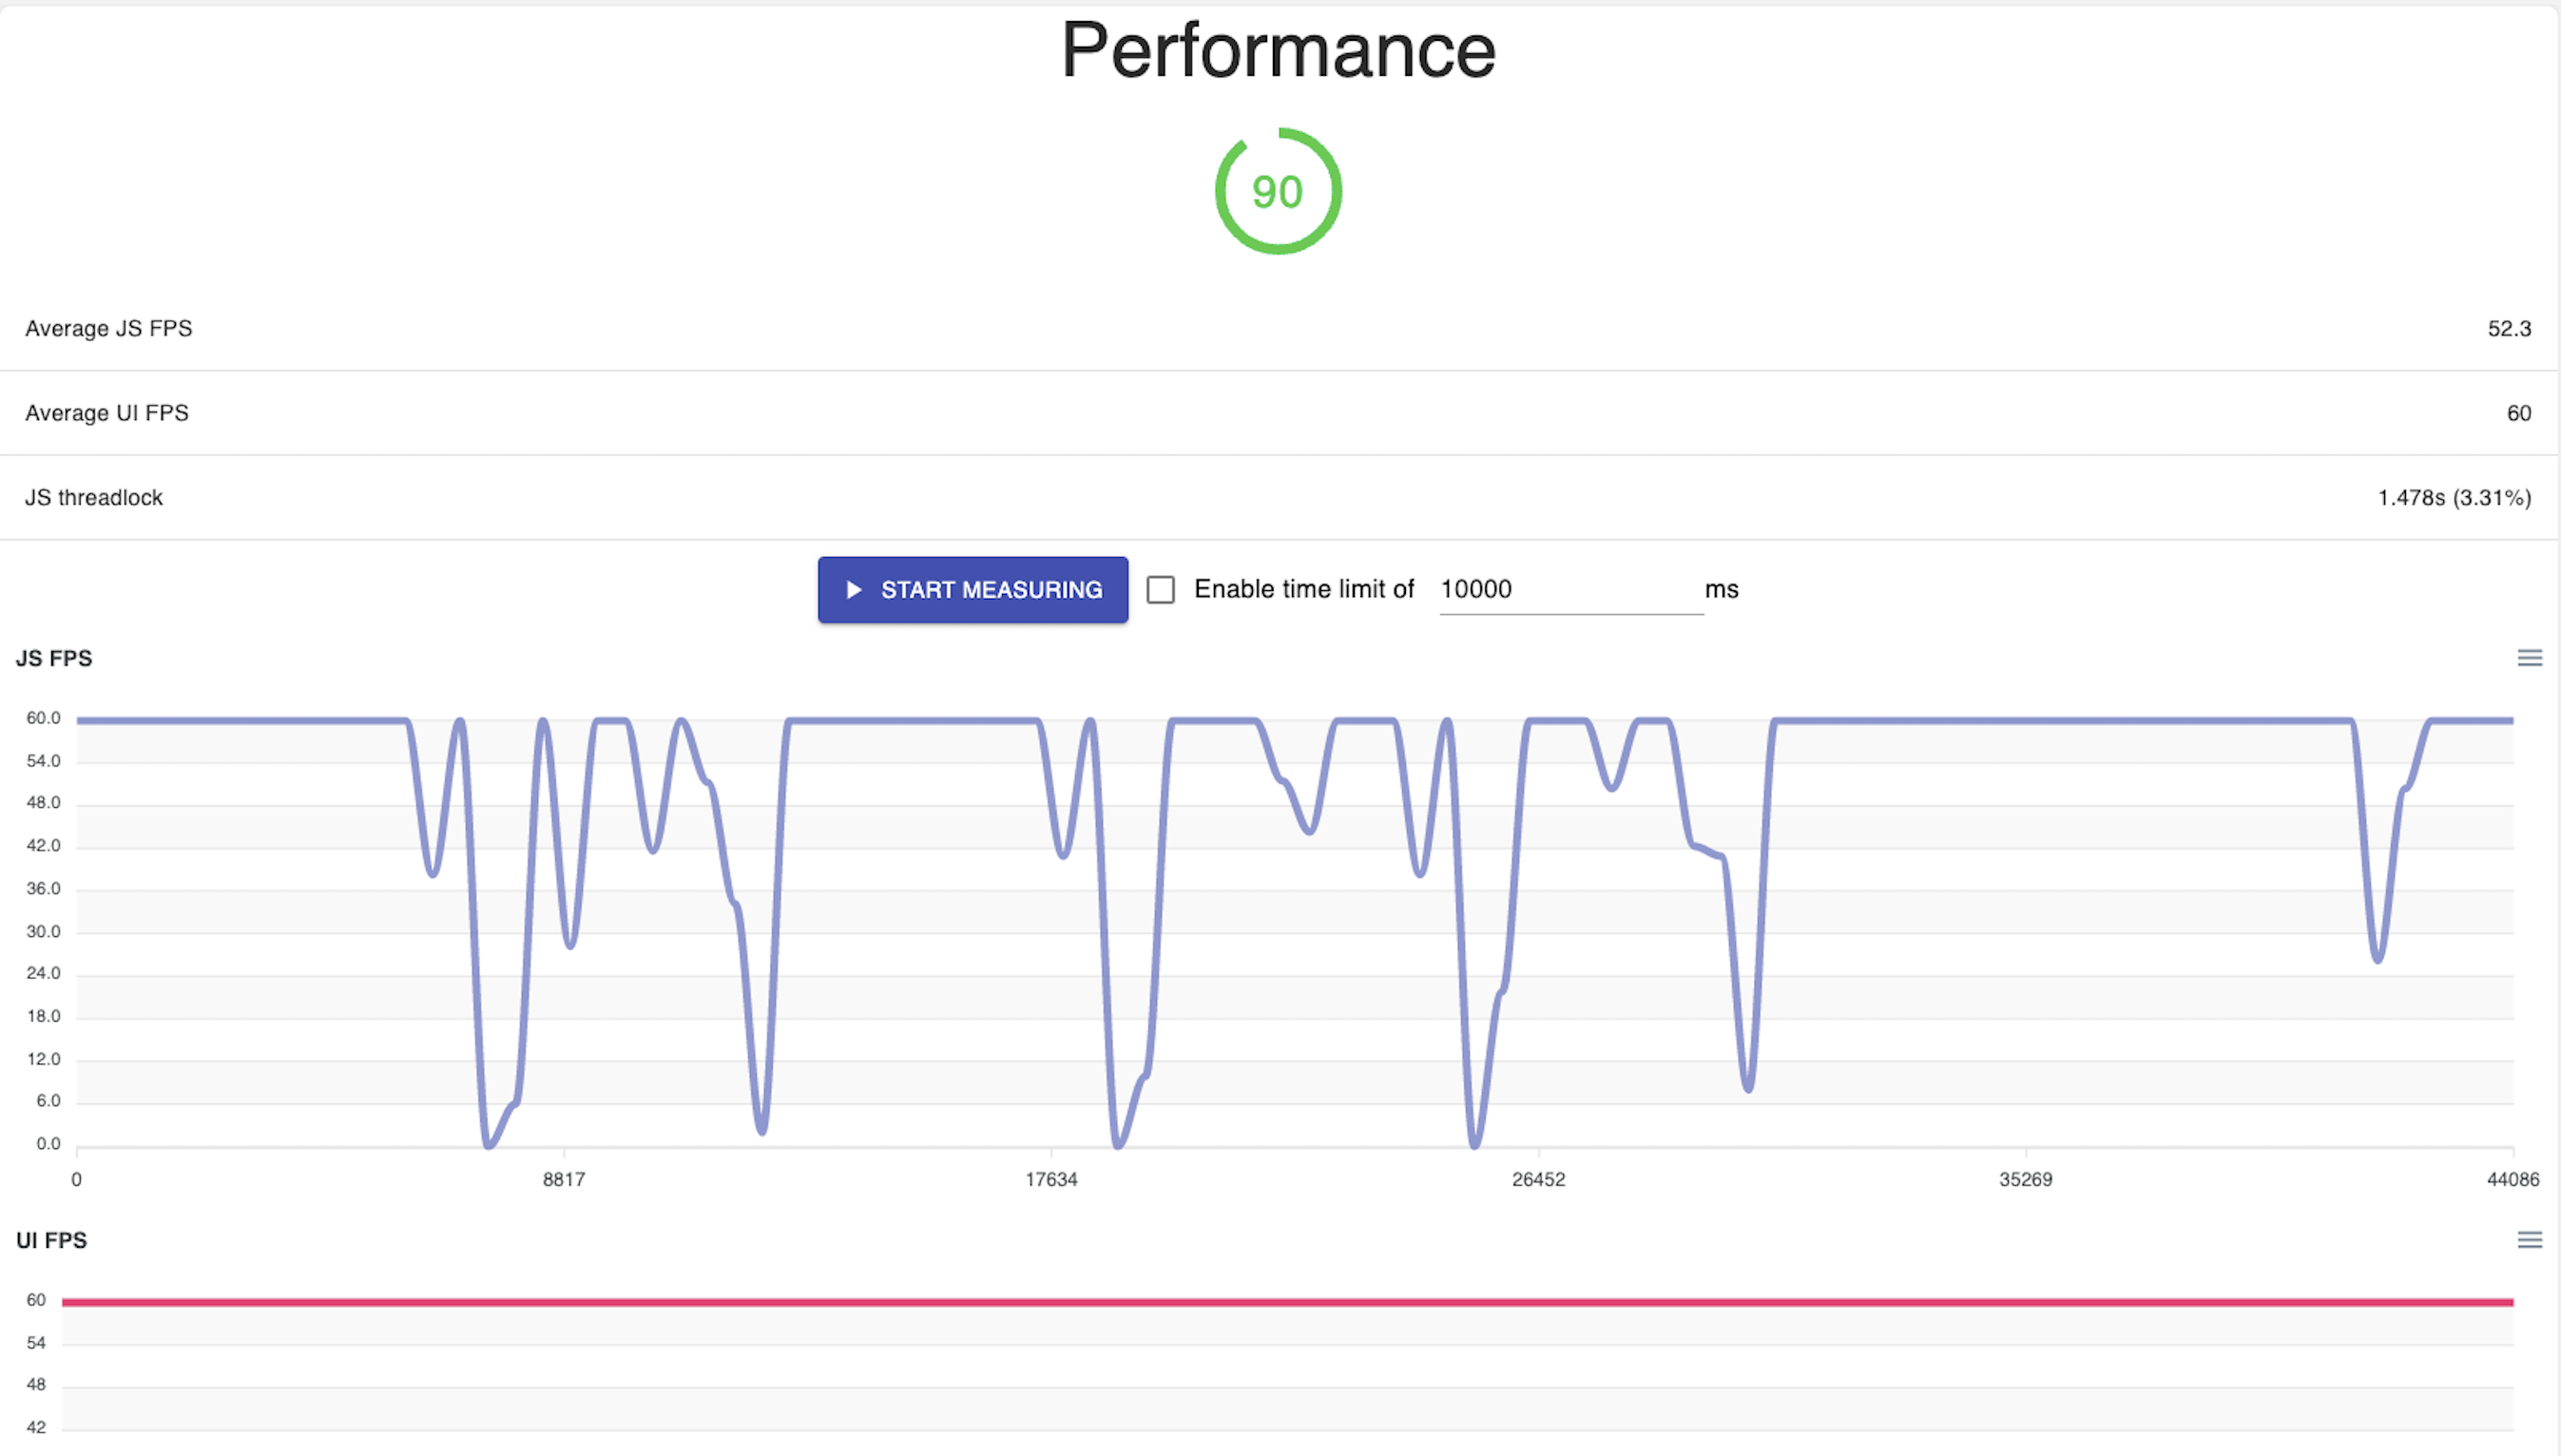
\includegraphics[width=6cm]{docs/images/chapterFive/fliperPerf.png} }}
\end{figure}

\chapter{Sistem za praćenje događaja u mobilnoj aplikaciji}

U savremenom poslovanju, praćenje poslovnih metrika igra ključnu ulogu u donošenju informisanih odluka i optimizaciji poslovnih odluka. Poslovne metrike omogućavaju kompanijama da prate performanse, identifikuju trendove i prepoznaju oblasti koje zahtevaju poboljšanja. U ovom poglavlju, fokusiraćemo se na značaj poslovnih metrika i predstaviti predlog za implementaciju sistema za praćenje događaja (eng, events) unutar React Native aplikacije.

Na primeru implementacije jednog ovakvog sistema razmatraćemo najbolje prakse za prikupljanje podataka u realnom vremenu, kako bi se obezbedilo tačno i pravovremeno praćenje ključnih indikatora performansi. Takođe, detaljno ćemo opisati korake za implementaciju skalabilnog i fleksibilnog sistema koji može da se prilagodi specifičnim potrebama kompanije, omogućavajući menadžmentu da donosi odluke zasnovane na preciznim i relevantnim informacijama. Na kraju, istražićemo načine za vizualizaciju i interpretaciju prikupljenih podataka, što će pomoći kompanijama da steknu dublji uvid u svoje operacije i značajno poboljšaju svoje performanse.

\section{Značaj poslovnih metrika}

Često, prilikom izrade softvera kraj se proglašava onog momenta kada su sve funkcionalnosti implementirane. Ovakav pristup je po pravilu pogrešan. Greška se ogleda u činjenici da ne postoji sistem koji nije moguće unaprediti. Takođe, često je veoma teško uočiti prostor za poboljšanje ukoliko nemamo mehanizme koji nam to omogućavaju. Mehanizam kome se najčešće pribegava jeste čuvanje svih relevantnih događaja u bazama podataka. Ovi događaji se kasnije obrađuju i iz tog oblika se izvlače poslovni zaključci koji će kasnije voditi ka definisanju prostora za poboljšanje i novim funkcionalnostima u sistemu.

\begin{figure}[h!]
\centering
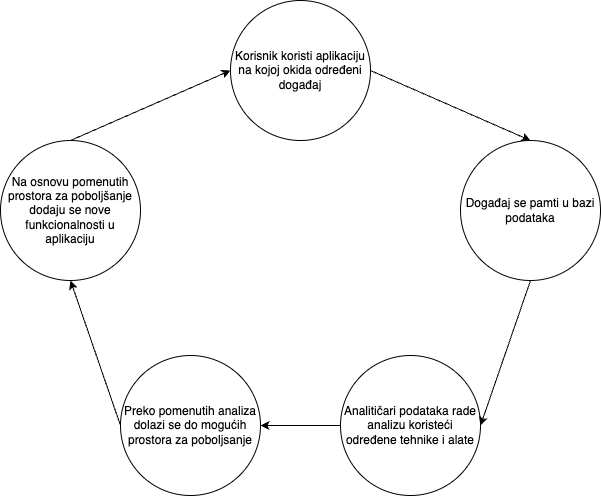
\includegraphics[scale=0.5]{docs/images/chapterSix/dataFlow.png}
\caption{Ciklus unapređivanja aplikacije}
\label{fig:dataFlow}
\end{figure}

Na slici 6.1 vidimo ciklus unapređivanje proizvoda. Na samom početku imamo proizvod koji radi i koji korisnik upotrebljava. Taj korisnik tokom korišćenja našeg proizvoda okida neki događaj i ta informacija se smešta u bazi podataka. Informacije iz baze koriste analitičari podataka kako bi došli do zaključaka preko kojih se definišu delovi proizvoda koji se mogu unaprediti. Preko ovih delova proizvoda i analiziranih podataka definišemo konkretne funkcionalnosti koje inženjer implementira. U ovom momentu ponovo kreće ciklus.

Da bismo bili u mogućnosti da sprovedemo sve ove korake u delo od esencijalnog značaja nam je da imamo sistem u okviru naše mobilne aplikacije koji će nam ovo omogućiti. Jedan takav sistem biće opisan u narednoj sekciji.

\section{Arhitektura sistema za prećenje događaja}

Na samom početku, pre pravljenja jednog ovakvog sistema neophodno je definisati koje probleme on treba da reši. Ovakav pristup je često veoma koristan jer nas podstiče da izađemo iz okvira implementacije i da se fokusiramo na ono što želimo da napravimo, odnosno na problem koji želimo da rešimo.
\newline
\newline
Osnovne funkcionalnosti sistema za praćenje događaja su:
\begin{itemize}
\item Lako dodavanje novih događaja
\item Mogućnost istovremenog upisivanja događaja na različite servise za čuvanje podataka
\item Lak način za unapređivanje događaja
\item Lako testiranje sistema pre puštanja na produkciju
\item Mogućnost da se na isti događaj reaguje na različite načine 
\end{itemize}

U nastavku ćemo predstaviti arhitekturu sistema koji zadovoljava sve gorepomenute kriterijume.

\subsection{Osnovni entiteti}

Prilikom razvijanja sistema za praćenje događaja uočavamo dva osnovna entiteta. U pitanju su događaj i pratilac događaja. Događaj nam je osnovni gradivni entitet na kom će se zasnivati sve dalje što budemo radili. On je implementiran kao interfejs koji mora imati polje eventName koje predstavlja ime tog događaja. Pored imena, svaki pojedinačni događaj može biti obogaćen dodatnim poljima koja bliže određuju isti. Ovo je omogućeno tako što je sam događaj ništa više nego TypeScript objekat. Dakle, imamo skup polja koja imaju neke vrednosti. 

\begin{figure}[h!]
\centering
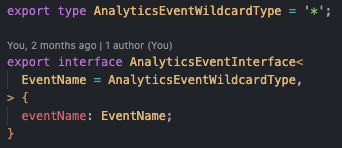
\includegraphics[scale=0.5]{docs/images/chapterSix/eventInterface.png}
\caption{Interfejs za događaj}
\label{fig:eventInterface}
\end{figure}

Drugi bitan entitet smo rekli da je pratilac događaja. On predstavlja klasu koja u sebi sadrži sve događaje na koje isti reaguje. Takođe, za svaki od tih događaja vezana je i funkcija koja nam govori kako će ovaj pratilac reagovati na taj specifičan događaj. Ovakvih pratilaca može u našem sistemu biti neograničeno i svaki od njih može da reaguje na proizvoljan broj događaja na proizvoljan način. Na primer, možemo imati jedan pratilac koji čemo koristiti za testiranje sistema i on će reagovati na sve događaja tako što će da ih loguje u konzolu. U isto vreme, možemo da imamo drugi pratilac koji će takođe reagovati na sve događaje, međutim, on će ih prosleđivati u našu bazu podataka.

\begin{figure}[h!]
\centering
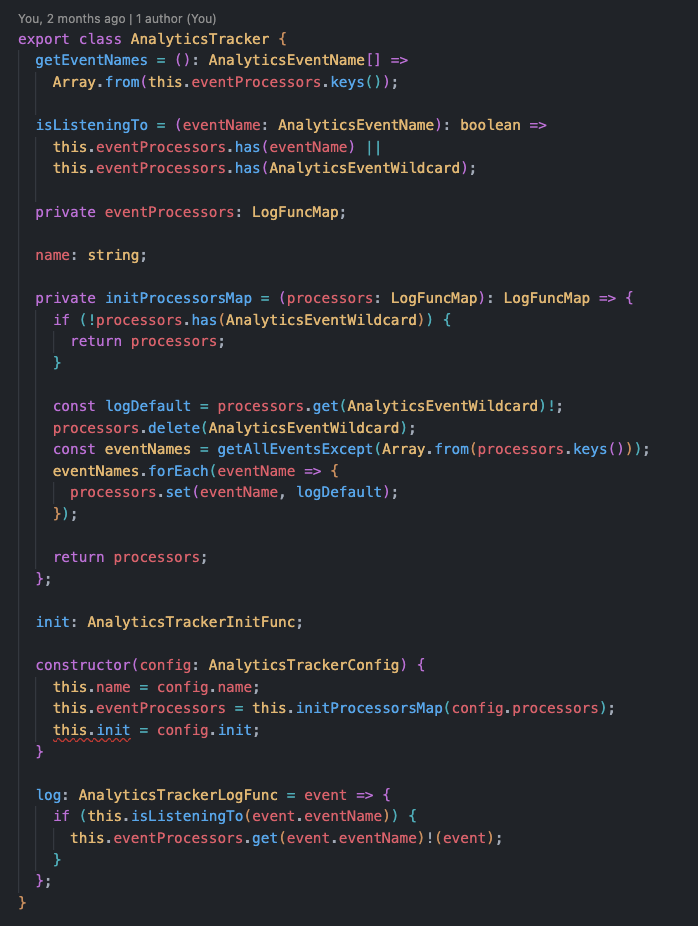
\includegraphics[scale=0.5]{docs/images/chapterSix/analyticsTracker.png}
\caption{Klasa za pratilac događaja}
\label{fig:analyticsTracker}
\end{figure}

Nakon što smo definisali ova dva entiteta potrebno nam je nešto što će da ih poveže i zapravo obezbedi željenu funkcionalnost. U našem slučaju to će da bude AnalyticsEventBus klasa. Ona će da bude realizovana kao obrazac Unikat (eng. Singleton). Dakle, kreiraće se samo jedna instanca ove klase i biće korišćena kroz celu aplikaciju. Ova klasa posedovaće niz svih pratilaca događaja koje smo kreirali. Takođe, omogućavaće dodavanje novih pratilaca. Glavna funkcionalnost ove klase biće funkcija za obradu nekog događaja. Kada se okine događaj, ova klasa će se pobrinuti da svaki pratilac koji treba da reaguje na taj događaj to zapravo i uradi. Kako sve to radi, videćemo malo kasnije.

\begin{figure}[h!]
\centering
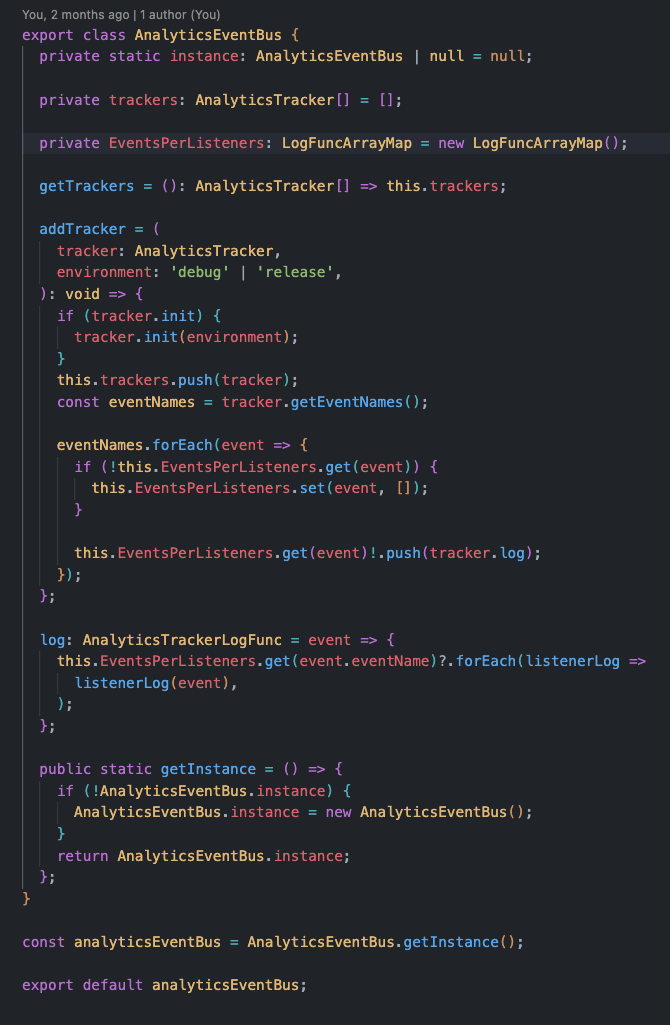
\includegraphics[scale=0.45]{docs/images/chapterSix/analyticsEventBus.png}
\caption{Glavna klasa za sistem za praćenje događaja}
\label{fig:analyticsEventBus}
\end{figure}

Na sledećoj slici biće prikazan UML dijagram koji definiše odnose između kreiranih klasa i interfejsa.

\begin{figure}[h!]
\centering
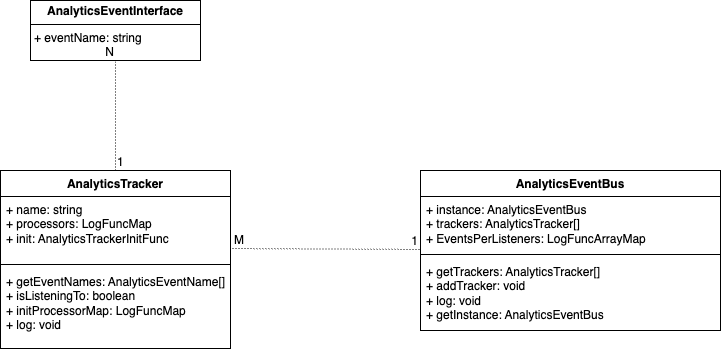
\includegraphics[scale=0.5]{docs/images/chapterSix/uml.png}
\caption{UML dijagram}
\label{fig:umlDiagram}
\end{figure}

\subsection{Primer korišćenja i funkcionisanja}

U ovoj sekciji biće prikazan način korišćenja prethodno kreiranog sistema. Takođe, biće detaljno objašnjeno kako ceo proces funkcioniše.

\begin{figure}[h!]
\centering
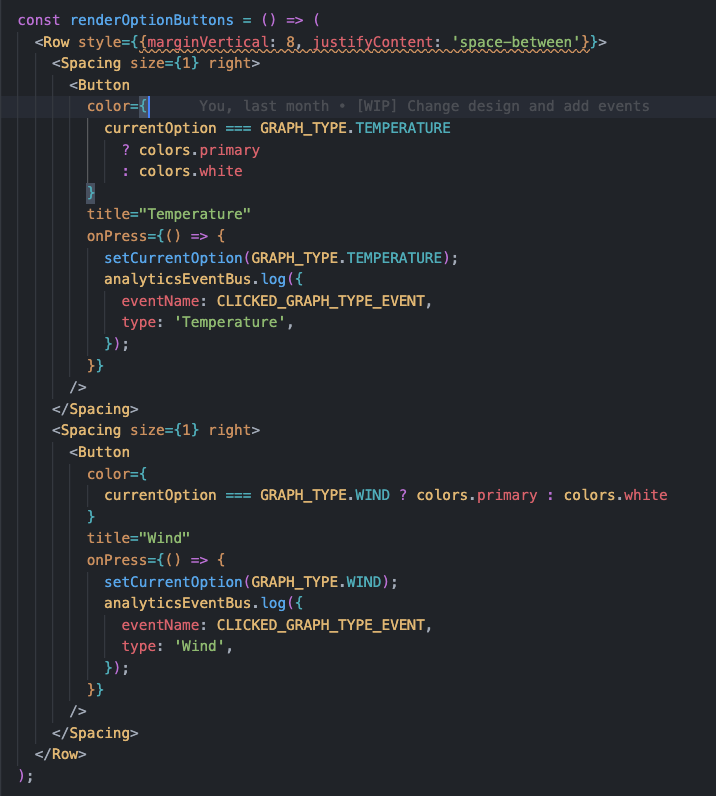
\includegraphics[scale=0.30]{docs/images/chapterSix/eventUsage.png}
\caption{Primer korišćenja događaja}
\label{fig:eventUsage}
\end{figure}

Na slici iznad vidimo kako se loguje jedan event. Tu dohvatamo instancu naše unikat klase analyticsEventBus. Nad ovom instancom klase pozivamo \textit{log} metodu kojoj prosleđujemo jedan konkretan događaj koji je potrebno da se loguje. Vidimo da naš događaj, pored obaveznog polja \textit{eventName} ima i polje \textit{type} koje ga bliže određuje. \newline

U ovom momentu, kreće da se izvršava \textit{log} metoda klase AnalyticsEventBus. Ranije smo pomenuli da svaki od pratilaca događaja, ukoliko reaguje na neki događaj mora da poseduje funkciju koja se poziva kada se okine taj događaj. U \textit{log} metodi dohvatamo sve funkcije koje treba da se pozovu za taj događaj. Dakle, prolazimo kroz sve pratioce događaja i ukoliko oni reaguju na naš događaj dodajemo funkciju u niz. Nakon ovoga prolazimo kroz dobijeni niz i pozivamo svaku funkciju iz istog pri čemu je parametar uvek isti, naš okinuti događaj. U konkretnoj implementaciji ovaj korak je optimizovan i ovaj niz se ne računa svaki put kada se događaj okine već samo prilikom dodavanja novog pratioca događaja. Kada se doda novi pratioc događaja, prolazimo kroz sve događaje na koje on reaguje i mapiramo ih u objekat koji je zajednički za sve pratioce. U ovom objektu ključevi su imena događaja, a vrednost su sve funkcije koje treba pozvati prilikom okidanja konkretnog događaja. \newline

Ovom optimizacijom se značajno štede performanse. Recimo da je broj događaja označen sa M, broj pratioca sa N i recimo da je okinuto P događaja. Ukoliko bismo koristili pristup koji je prvi opisan, prilikom okidanja P događaja svaki put bismo preračunavali niz funkcija koje treba da se pozovu. Jedno računanje je složenosti O(N*M) jer svaki put prolazimo kroz N pratioca i za svakog pratioca prolazimo kroz M događaja. Dakle, ukupna složenost kreiranja bi bila O(P*N*M). Dok bismo u drugom pristupu imali složenost O(N*M) jer računanje radimo samo jednom, prilikom dodavanja pratioca.

\chapter{Sistem za praćenje grešaka unutar aplikacije}

Pored prethodno pomenutih sistema za merenje performansi i poslovnih metrika aplikacije, od esencijalnog značaja nam je da postavimo sistem za praćenje grešaka. Realnost je da većina aplikacija ima greške, odnosno da funkcionisanje odstupa od specifikacije. Veoma je bitno da možemo to da uočimo na sistematičan način i da adresiramo kako bismo u budućnosti otklonili ta neželjena ponašanja i obezbedili fluidno iskustvo za korisnike. Ovaj problem je veoma izazovan jer su aplikacije često veoma velike i većina slučaja upotrebe nije trivijalna i potrebno je da se ispuni priličan broj uslova da bismo to reprodukovali. Sve ovo testiranje i pronalaženje ovih problema čini težim. U svrhe olakšavanja pronalaženja problema unutar aplikacije ćemo odraditi integraciju sistema Sentry. Ovaj sistem smo već koristili u poglavlju o performansama. Tada smo odradili integraciju koja nam je dozvolila da pratimo performansne metrike. Sada će nam ta ista integracija omogućiti da beležimo sve greške koje su se dogodile u našoj aplikaciji uz propratne informacije koje će nam omogućiti da odradimo u kom delu sistema se problem dešava.

\subsection{Kako ova integracija funkcioniše?}

Kao što smo i pre rekli, biblioteka Sentry integriše se u React Native mobilnoj aplikacije tako što se cela aplikacija obmotava samim SDK-jom (eng. Software development kit). Mi smo to uradili u App.tsx fajlu. Dakle, kada se desi neka greška unutar naše aplikacije ona će biti propagirana do samog vrha. Biblioteka Sentry će registrovati grešku, pridružiće joj što je moguće više parametara kako bi razvojni tim mogao da zaključi šta se zapravo desilo što brže i efikasnije. Nakon što je ovo odrađeno, ta greša se salje na Sentry plaformu gde ćemo je mi zapravo videti i dalje analizirati.

\begin{figure}[h!]
\centering
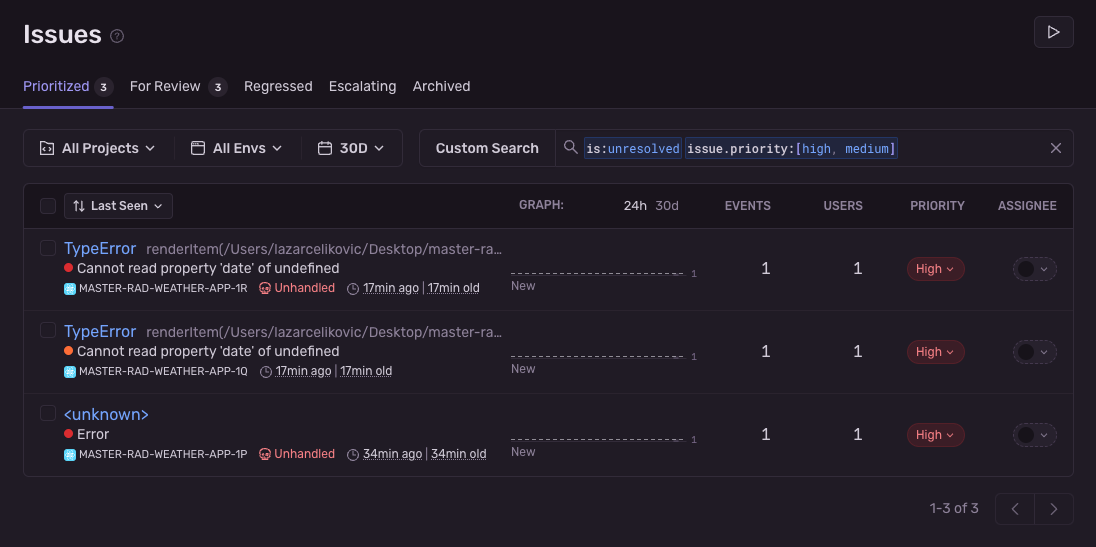
\includegraphics[scale=0.4]{docs/images/chapterSeven/sentryErrorLogs.png}
\caption{Primer liste grešaka na plaformi Sentry}
\label{fig:sentryErrorList}
\end{figure}

Na slici iznad vidimo glavnu stranicu platofrme Sentry. Na istoj su izlistane sve greške koje su se desile unutar naše aplikacije. U nastavku ćemo analizirati glavne funkcionalnosti.

\section{Funkcionalnosti platforme Sentry}

Kao što smo videli na slici 7.1, platforma Sentry nam pruža ogromnu količinu podataka o svakoj pojedinačnoj grešci koje je logovana na istoj. Na glavnoj stranici su izlistane sve greške koje su se desile unutar aplikacije i date su nam najosnovnije informacije o svakoj pojedinačnoj grešci. Ove informacije uključuju momenat dešavanja, naziv i opis greške, broj pojavljivanja greške i broj korisnika koji su je iskusili. Takođe, prikazan nam je prioritet greške kao i osoba kojoj je dodeljeno rešavanje. Ovo polje je posebno interesantno jer nam sama plaforma omogućava dodatnu integraciju sa servisom GitHub. Uz pomoć ovog servisa ovo polje će automatksi biti popunjeno, odnosno rešavanje problema biće dodeljeno onom članu razvojnog tima koji je poslednji vršio izmenu linije koda u kojoj se desila greška. \newline

Zanimljiviji i svakako korisniji deo ove plaforme jeste sama stranica o grešci. Klikom na svaku pojedinačnu grešku bićemo navigirani na posebnu stranicu gde ćemo dobiti sve dostupne informacije o istoj kako bismo mogli da je rešimo. Ova stranica je veoma obimna i pruža ogromnu količinu informacija, tako da ćemo da je podelimo na manje celine i tako ih analiziramo.

\subsection{Najosnovnije informacije o grešci}

Prva sekcija na stranici daje nam najosnivnije informacije o grešci koju analiziramo. Tu mozemo da vidimo sam tekst greške, fajl u kome se greška dogodila, broj pojavljivanja greške kao i broj korisnika kod kojih se greška manifestovala. Takođe, vidimo broj broj pojavljivanja greške kako u poslednja 24 časa, tako i u poslednjih mesec dana, kao i podatke o verziji aplikacije u kojoj smo prvi i poslednji put uočili grešku. Pomoću ovih informacija možemo da odredimo interni prioritet greške i da odlučimo da li ćemo prioritizovati njeno rešavanje ili ne.

\begin{figure}[h!]
\centering
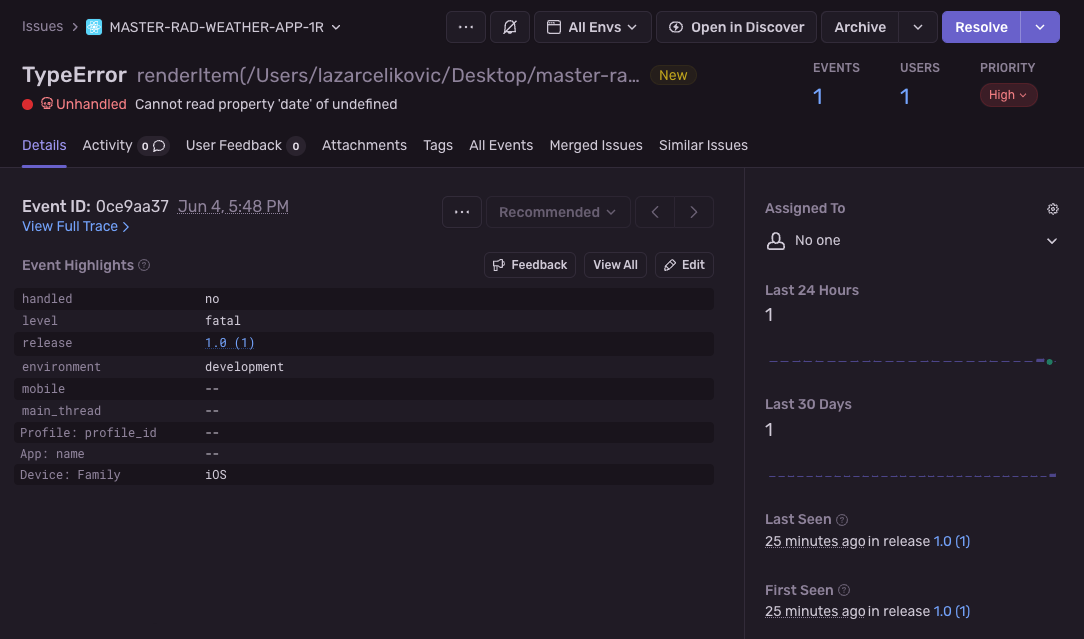
\includegraphics[scale=0.4]{docs/images/chapterSeven/sentryErrorBasicData.png}
\caption{Osnovni podaci o grešci}
\label{fig:sentryErrorBasicInfo}
\end{figure}

Nakon ovih informacija, vidimo deo koda u kom se greška dogodila. Ovo je veoma korisna informacija jer sužava pretragu i daje nam ključne informacije kako bismo mogli da krenemo sa procesom debagovanja. Ovde takođe imamo opciju da pogledamo celu putanju greške (eng. stacktrace). Ova opcija je naročito korisna kada je u pitanju greška unutar nekog eksternog sistema ili biblioteke. U tom slučaju, sama greška se manifestuje kod nas u aplikaciji, ali je rešavanje potrebno sprovesti van iste. 

\begin{figure}[h!]
\centering
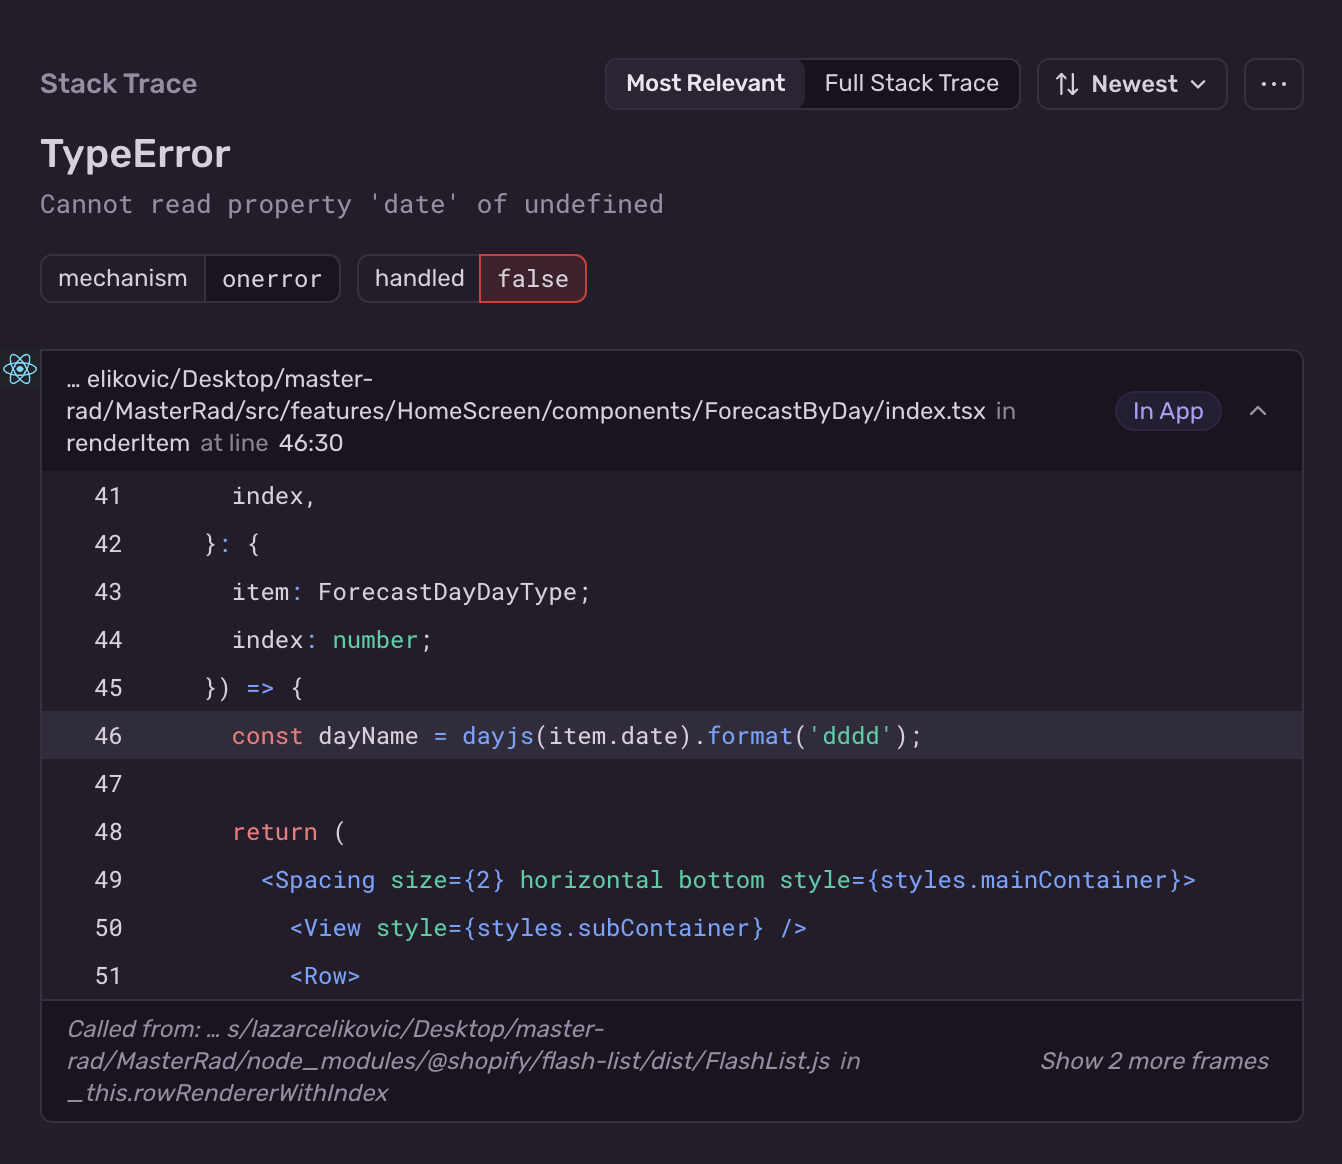
\includegraphics[scale=0.4]{docs/images/chapterSeven/SentyErrorStacktrace.png}
\caption{Informacije o delu koda gde se greška javlja}
\label{fig:sentryStacktrace}
\end{figure}

\subsection{Koncept mrvica hleba}

Mrvice hleba (eng. breadcrumbs) unurar sistema Sentry predstavljaju sekvencu događaja ili akcija koji su se dogodili neposredno pre greške unutar naše aplikacije. Koncept je potekao od ostavljanja mrvica hleba koje će nam pomoći da dođemo do tačke kada je nešto krenulo po zlu. Ove mrvice mogu biti logovane automatski, ali takođe mi možemo dodati naše lične. Pomoću njih olakšavamo posao kako sebi tako i razvojnom timu prilikom reprodukcije i debagovanja greške. Dakle, u ovoj sekciji možemo da pratimo tačnu interakciju korisnika sa našom aplikacijom pre nego što je došlo do greške. Platforma Sentry prikazuje nam API pozive koji su okinuti, interakciju sa elementima korisničkog interfejsa (klik na dugme, selektovanje radio dugmeta, popunjavanje tekstualnog polja, ...). Ove informacije su od ključnog značaja kako bismo mogli da razumemo slučaj upotrebe kao i tok akcija koje dovode do nekog problema. \newline

\newline

\begin{figure}[h!]
\centering
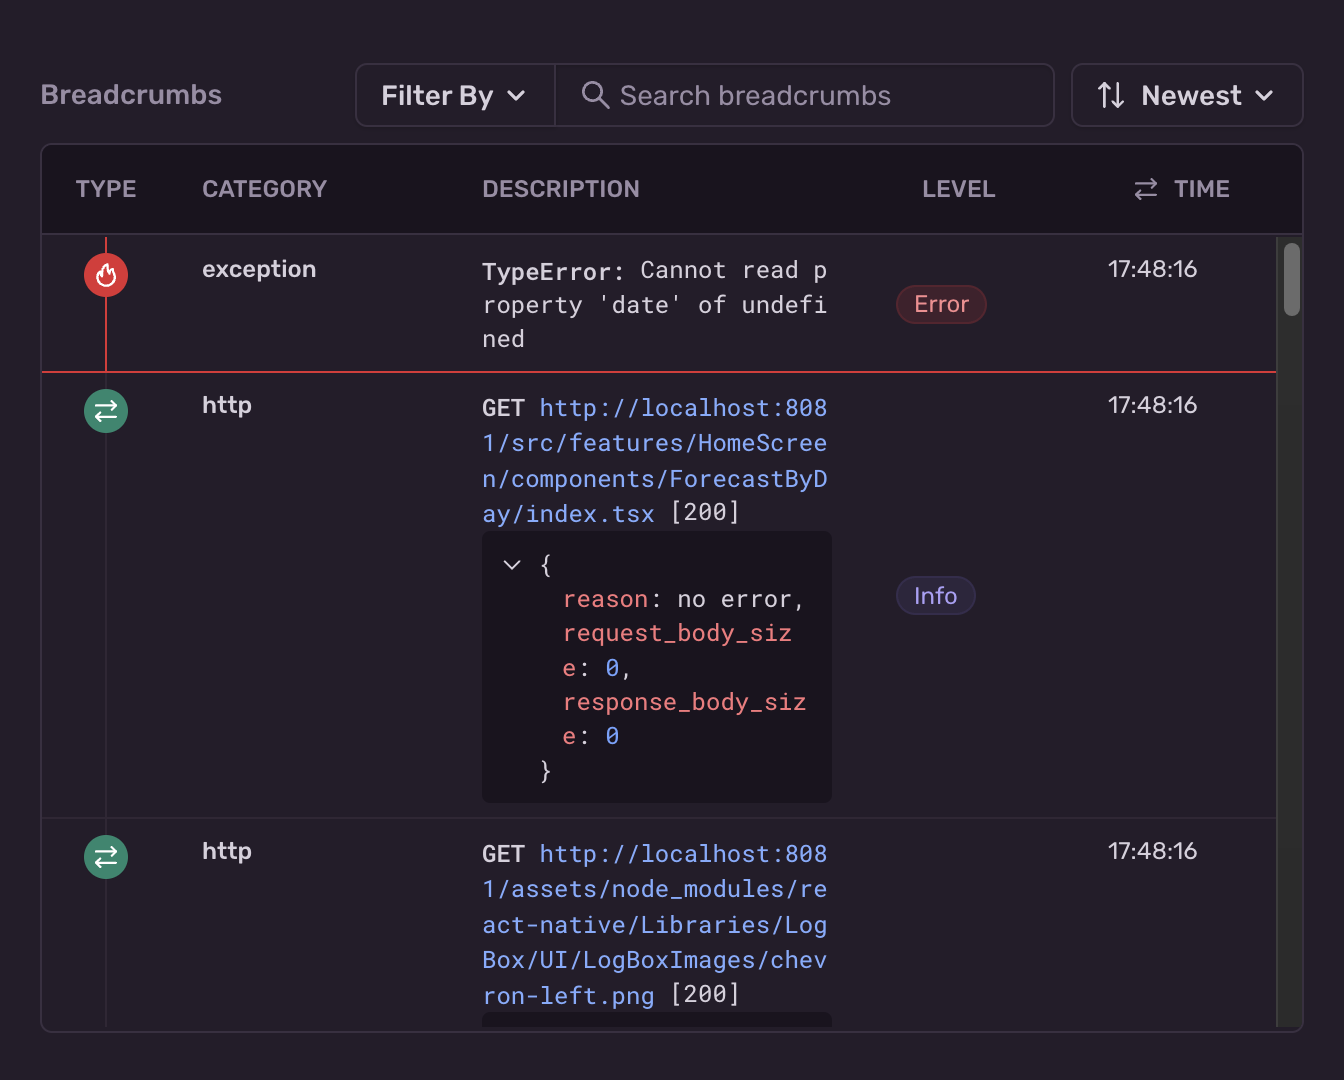
\includegraphics[scale=0.4]{docs/images/chapterSeven/SentryBreadcrumbs.png}
\caption{Breadcrumbs}
\label{fig:sentryBreadcrumbs}
\end{figure}

Često, greške koje se desavaju unutar sistema se ne nalaze u glavnim tokovima korišćenja (eng. flows), već u nekim specifičnim slučajevima upotrebe. Na primer, korisnik je kliknuo na push notifikaciju ili deeplink i preko neke od ovih funkcionalnosti bio navigiran na određenu stranicu i tom prilikom dešava se greška na ovoj stranici. Kada razvojni tim pokuša da reprodukuje ovo ponašanje greška se ne desi. Ovo je veoma čest slučaj i poenta je u tome da u velikim sistemima postoji mnogo načina da se dodje do istog dela sistema i praktično je nemoguće testirati ih sve. U ovim situacijama nam može biti korisno da dodamo naše lične breadcrumbs kako bismo olakšali određivanje tačne putanje kojom je korisnik došao do greške. Sentry plaforma nam pruža ovu mogućnost.

\begin{figure}[h!]
\centering
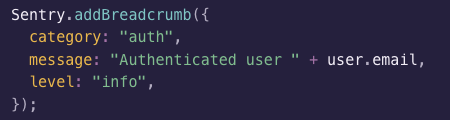
\includegraphics[scale=0.8]{docs/images/chapterSeven/addBreadcrumb.png}
\caption{Dodavanje novog breadcrumb-a}
\label{fig:addBreadcrumb}
\end{figure}

\subsection{Informacije o uređaju}

Neretko, same greške imaju povezanost sa trenutnim stanjem uređaja. Na primer, ukoliko je internet konekcija slaba može doći do povećanog vremena čekanja za informacije sa servera ili čak do situacija kada te informacije uopšte ne stignu nazad. Takođe, ukoliko je novi baterije pri kraju to takođe može da izazove razne probleme u funkcionisanju aplikacije. Platforma Sentry nam pruža i ove informacije.

\begin{figure}[h!]
\centering
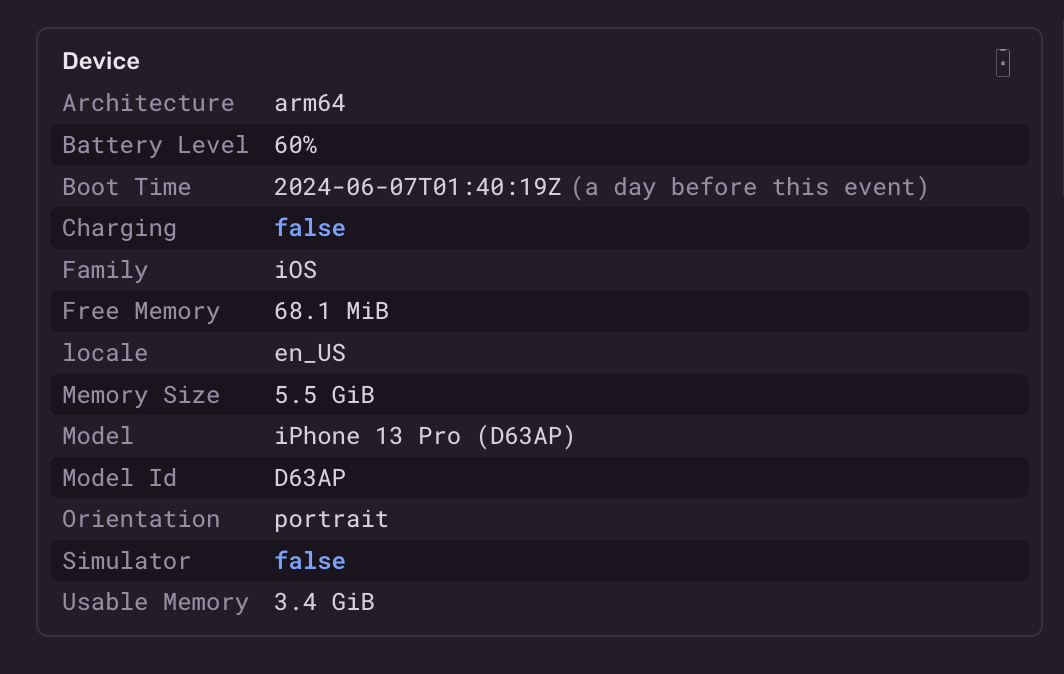
\includegraphics[scale=0.8]{docs/images/chapterSeven/deviceInfo.png}
\caption{Informacije o uređaju}
\label{fig:deviceInfo}
\end{figure}

\section{Poboljšana arhitektura za praćenje grešaka}

Sada, kada smo videli šta nam sve plaforma Sentry nudi i kako možemo da odradimo osnovnu inicijalizaciju vreme je da razmislimo o unapređivanju postojećeg rešenja. Za početak, potrebno je da definišemo koje sve tipove grešaka želimo da pratimo. To su sve one greške do kojih dolazi do prekida rada aplikacije ili do neželjenih ponašanja u korisničkom iskustvu. Ti tipovi grešaka su:

\begin{itemize}
\item Neobrađene greške (eng. ungandled errors) - ove greške se dešavaju u momentu kada aplikacija naiđe na grešku i ne zna kako da je obradi. Ove greške nisu veoma česte, ali ukoliko se dese veoma često dovode do potpunog prestanka rada aplikacije.
\item JavaScript greške (eng. JS erros) - ove greške predstavljaju najveći deo svih grešaka unutar React Native aplikacija. U pitanju su stvari kao što su sintaksne greške, pristupanju poljima objekata pri čemu sam objekat ima vrednost undefined.
\item Mrežne greške (eng. Network errors) - ova grupa obuhvata sve greške koje se događaju usled nemogućnosti aplikacije da komunicira sa serverom. Kao što smo ranije pominjali, to su problemi sa slabom internet konekcijom, ali i potpunim odsustvom mreže.
\end{itemize}

Kada smo ovo odradili, mozemo da napravimo omotač oko naše React Native aplikacije koje će nam služiti da obrađuje sve greške koje se dese unutar aplikacije na način koji mi definišemo. Ovo ćemo realizovati preko ErrorBoundary komponente. Ovo je jedan od standardnih obrazaca kod React i React Native aplikacije. U pitanju je komponenta koje služi kao omotač oko cele aplikacije. Kada se greška dogodi, biva propagirana kroz od dna do vrha stabla komponenti i na kraju biva uhvaćena u okviru ovog omotača. Mi tu obrađujemo i normalizujemo grešku i šaljemo je na Sentry plaformu. \newline

\newline

Sentry nam pruža ugrađenu podršku za ovo. Na slici ispod ćemo videti kako bi izgledala implementacija.


% ------------------------------------------------------------------------------
\chapter{Zaključak}
% ------------------------------------------------------------------------------
\pangrami

\pangrami

% ------------------------------------------------------------------------------
% Literatura
% ------------------------------------------------------------------------------
\literatura

% ==============================================================================
% Završni deo teze i prilozi
\backmatter
% ==============================================================================

% ------------------------------------------------------------------------------
% Biografija kandidata
\begin{biografija}
  \textbf{Vuk Stefanović Karadžić} (\emph{Tršić,
    26. oktobar/6. novembar 1787. — Beč, 7. februar 1864.}) bio je
  srpski filolog, reformator srpskog jezika, sakupljač narodnih
  umotvorina i pisac prvog rečnika srpskog jezika.  Vuk je
  najznačajnija ličnost srpske književnosti prve polovine XIX
  veka. Stekao je i nekoliko počasnih mastera.  Učestvovao je u
  Prvom srpskom ustanku kao pisar i činovnik u Negotinskoj krajini, a
  nakon sloma ustanka preselio se u Beč, 1813. godine. Tu je upoznao
  Jerneja Kopitara, cenzora slovenskih knjiga, na čiji je podsticaj
  krenuo u prikupljanje srpskih narodnih pesama, reformu ćirilice i
  borbu za uvođenje narodnog jezika u srpsku književnost. Vukovim
  reformama u srpski jezik je uveden fonetski pravopis, a srpski jezik
  je potisnuo slavenosrpski jezik koji je u to vreme bio jezik
  obrazovanih ljudi. Tako se kao najvažnije godine Vukove reforme
  ističu 1818., 1836., 1839., 1847. i 1852.
\end{biografija}
% ------------------------------------------------------------------------------

\end{document}
